% !Mode:: "TeX:UTF-8"
\def\usewhat{xelatex}
\PassOptionsToPackage{no-math}{fontspec}
\documentclass[12pt,openany,oneside]{book}
% !Mode:: "TeX:UTF-8"
\usepackage{graphicx}
\usepackage[export]{adjustbox}
\usepackage{eso-pic}
\usepackage[a4paper,margin=2.6cm,head=6mm,headsep=6.5mm,footskip=1.1cm]{geometry}

\usepackage{titlesec}
\usepackage{titletoc}
\usepackage{fancyhdr}
\ifdefined\XeTeXversion
  \PassOptionsToPackage{fontset=none}{ctex}
\fi
\usepackage[UTF8]{ctex}
\usepackage{color}
\usepackage{amsmath}
\usepackage{amssymb}
\usepackage{newtxmath}
\usepackage{placeins}
\usepackage{wrapfig}
\usepackage{needspace}
\usepackage{multirow}
\usepackage{booktabs}
\usepackage{longtable}
\usepackage{tabularx}
\usepackage{subfigure}
\usepackage[subfigure]{ccaption}
\usepackage[sort&compress,numbers]{natbib}
\usepackage{enumitem}
\usepackage{calc}
\usepackage{float}
\usepackage{bm}
\usepackage[amsmath,thmmarks,hyperref]{ntheorem}
\usepackage{CJKnumb}
\usepackage{indentfirst}
\usepackage{tikz}
\usepackage{xcolor}
\usepackage{listings}

\newcommand{\tabincell}[2]{\begin{tabular}{@{}#1@{}}#2\end{tabular}}
\newcommand{\shot}[2][0.94\linewidth]{{\setlength{\fboxsep}{0pt}\setlength{\fboxrule}{0.45pt}\fcolorbox{black!25}{white}{\includegraphics[width=#1]{#2}}}}
\newcommand{\shotbox}[2]{\setlength{\fboxsep}{0pt}\setlength{\fboxrule}{0.45pt}\fcolorbox{black!25}{white}{\includegraphics[#1]{#2}}}

\lstdefinelanguage{JavaScript}{
  keywords={const,let,var,function,return,if,else,for,of,in,while,async,await,try,catch,new,true,false,null,undefined,export,import,from,default},
  sensitive=true,
  comment=[l]{//},
  morecomment=[s]{/*}{*/},
  morestring=[b]',
  morestring=[b]",
  morestring=[b]`
}
\lstset{numbers=left,
language=Python,
numberstyle=\tiny\color[RGB]{150,150,150},
numbersep=7pt,
extendedchars=false,
showstringspaces=false,
breakatwhitespace=false,
breaklines=true,
captionpos=b,
keywordstyle=\bfseries\color{black},
commentstyle=\color{black!65},
stringstyle=\color{black},
frame=single,
framerule=0.4pt,
rulecolor=\color[RGB]{205,205,205},
backgroundcolor=\color[RGB]{248,248,248},
framesep=3pt,
xleftmargin=1.4em,
framexleftmargin=.7em,
columns=fullflexible,
keepspaces=true,
basicstyle=\linespread{1.0}\ttfamily\fontsize{8.5bp}{10.8bp}\selectfont,
tabsize=2
}
\makeatletter
\let\ReportListingFrameExit\lst@frameExit
\def\lst@frameExit{\nobreak\ReportListingFrameExit}
\makeatother
\renewcommand{\lstlistingname}{代码}

\usepackage{array}
\newcommand{\PreserveBackslash}[1]{\let\temp=\\#1\let\\=\temp}
\newcolumntype{C}[1]{>{\PreserveBackslash\centering}p{#1}}
\newcolumntype{R}[1]{>{\PreserveBackslash\raggedleft}p{#1}}
\newcolumntype{L}[1]{>{\PreserveBackslash\raggedright}p{#1}}

\usepackage{hyperref}
\hypersetup{
    unicode=true,
    pdfborder={0 0 0},
    bookmarksnumbered=true,
    bookmarksopen=true,
    colorlinks=false,
}

% 允许正文中的长标识符自然断行，避免整段中文行距或字距被拉散
\ExplSyntaxOn
\tl_new:N \l__tju_tt_tl
\regex_const:Nn \c__tju_camel_regex { ([a-z0-9]) ([A-Z]) }
\regex_const:Nn \c__tju_punct_regex { ([\./:\-]) }
\regex_const:Nn \c__tju_us_regex { (\c{_}) }
\cs_new_protected:Npn \tju_tt_breakable:n #1
  {
    \tl_set:Nn \l__tju_tt_tl {#1}
    \regex_replace_all:NnN \c__tju_camel_regex { \1 \c{penalty} 100 \c{relax} \2 } \l__tju_tt_tl
    \regex_replace_all:NnN \c__tju_punct_regex { \1 \c{penalty} 50 \c{relax} } \l__tju_tt_tl
    \regex_replace_all:NnN \c__tju_us_regex { \1 \c{penalty} 50 \c{relax} } \l__tju_tt_tl
    \tl_use:N \l__tju_tt_tl
  }
\cs_set_eq:NN \tjuttbreak \tju_tt_breakable:n
\ExplSyntaxOff
\usepackage{letltxmacro}
\LetLtxMacro{\tjuorigtexttt}{\texttt}
\DeclareRobustCommand{\texttt}[1]{\tjuorigtexttt{\tjuttbreak{#1}}}
\AtBeginDocument{\pdfstringdefDisableCommands{\def\texttt#1{#1}}}

\usepackage{caption}
\DeclareCaptionFont{reportcaption}{\fontsize{10.5bp}{12.6bp}\selectfont}
\captionsetup{font=reportcaption,labelfont=bf,skip=6pt}
\captionsetup[table]{position=top,skip=6pt}
\captionsetup[figure]{position=bottom,skip=6pt}

% 紧凑实验摘录与对比信息卡（左侧细色条 + 浅灰底衬，避免正文堆砌大表格）
\definecolor{zwaccent}{HTML}{4A39B8}
\definecolor{zwtint}{HTML}{F7F7FC}
\definecolor{zwborder}{HTML}{DCDCE8}
\newcommand{\CaseCard}[2]{%
  \par\smallskip\noindent
  \begin{tikzpicture}
    \node[inner xsep=9pt, inner ysep=6.5pt, text width=\dimexpr\linewidth-20pt\relax,
          fill=zwtint, draw=zwborder, line width=0.45pt, rounded corners=1.5pt, align=justify] (box) {%
      {\setlength{\parfillskip}{0pt plus 1fil}\setlength{\parindent}{0pt}%
       \fontsize{10.5bp}{13.6bp}\selectfont\textbf{\color{zwaccent}#1}\par\vspace{2.5pt}#2}%
    };
    \draw[zwaccent, line width=2.2pt] (box.north west) -- (box.south west);
  \end{tikzpicture}\par\smallskip
}
\setlength{\columnsep}{12pt}


\makeatletter

% !Mode:: "TeX:UTF-8"
\newcommand{\ReportTriangleListFont}{}
\makeatletter
\RequirePackage{xeCJK}
\IfFontExistsTF{Times New Roman}{%
  \setmainfont[BoldFont={Times New Roman Bold}]{Times New Roman}
  \setsansfont[BoldFont={Times New Roman Bold}]{Times New Roman}
  \setmonofont[BoldFont={Liberation Mono Bold}]{Liberation Mono}
}{%
  \setmainfont{texgyretermes-regular.otf}[BoldFont=texgyretermes-bold.otf,ItalicFont=texgyretermes-italic.otf]
  \setsansfont{texgyretermes-regular.otf}[BoldFont=texgyretermes-bold.otf]
  \setmonofont{Liberation Mono}
}
\setCJKmainfont[BoldFont=FandolSong-Bold.otf]{FandolSong-Regular.otf}
\setCJKsansfont[BoldFont=FandolHei-Bold.otf]{FandolHei-Regular.otf}
\setCJKmonofont[BoldFont=FandolSong-Bold.otf]{FandolSong-Regular.otf}
\setCJKfamilyfont{song}[BoldFont=FandolSong-Bold.otf]{FandolSong-Regular.otf}
\setCJKfamilyfont{fs}[AutoFakeBold=2]{FandolFang-Regular.otf}
\setCJKfamilyfont{kai}[AutoFakeBold=2]{FandolKai-Regular.otf}
\setCJKfamilyfont{hei}[BoldFont=FandolHei-Bold.otf]{FandolHei-Regular.otf}
\setCJKfamilyfont{coverbody}[BoldFont=FandolSong-Bold.otf]{FandolSong-Regular.otf}
\setCJKfamilyfont{coversong}[BoldFont=FandolSong-Bold.otf]{FandolSong-Regular.otf}
\xeCJKsetup{CheckSingle=true,WidowPenalty=10000}

\newcommand{\song}{\CJKfamily{song}}
\newcommand{\fs}{\CJKfamily{fs}}
\newcommand{\kai}{\CJKfamily{kai}}
\newcommand{\hei}{\CJKfamily{hei}\sffamily\bfseries}
\newcommand{\coverbody}{\CJKfamily{coverbody}}

\DeclareSymbolFont{operators}{TU}{\rmdefault}{m}{n}
\SetSymbolFont{operators}{bold}{TU}{\rmdefault}{b}{n}
\DeclareMathAlphabet{\mathrm}{TU}{\rmdefault}{m}{n}
\makeatother

\newcommand{\yihao}{\fontsize{26pt}{26pt}\selectfont}
\newcommand{\xiaoyi}{\fontsize{24pt}{24pt}\selectfont}
\newcommand{\erhao}{\fontsize{22pt}{1.25\baselineskip}\selectfont}
\newcommand{\xiaoer}{\fontsize{18pt}{18pt}\selectfont}
\newcommand{\sanhao}{\fontsize{16pt}{16pt}\selectfont}
\newcommand{\xiaosan}{\fontsize{15pt}{15pt}\selectfont}
\newcommand{\sihao}{\fontsize{14pt}{14pt}\selectfont}
\newcommand{\xiaosi}{\fontsize{12pt}{12pt}\selectfont}
\newcommand{\wuhao}{\fontsize{10.5pt}{10.5pt}\selectfont}
\newcommand{\xiaowu}{\fontsize{9pt}{9pt}\selectfont}
\newcommand{\liuhao}{\fontsize{7.5pt}{7.5pt}\selectfont}

\newcommand{\ReportTriangle}{\raisebox{0.08ex}{\scalebox{1.25}{\ensuremath{\triangleright}}}}
\setitemize{label=\ReportTriangle,leftmargin=2.6em,itemsep=0.15em,partopsep=0em,parsep=0em,topsep=0.2em,before=\setlength{\parfillskip}{0pt plus 0.80\linewidth}}
\setenumerate{leftmargin=2.6em,itemsep=0.15em,partopsep=0em,parsep=0em,topsep=0.2em,before=\setlength{\parfillskip}{0pt plus 0.80\linewidth}}

\makeatletter
\renewcommand\normalsize{
  \@setfontsize\normalsize{12bp}{14.4bp}
  \setlength\abovedisplayskip{4pt}
  \setlength\abovedisplayshortskip{4pt}
  \setlength\belowdisplayskip{\abovedisplayskip}
  \setlength\belowdisplayshortskip{\abovedisplayshortskip}
  \let\@listi\@listI}
\def\defaultfont{\renewcommand{\baselinestretch}{1.25}\normalsize\selectfont}
\XeTeXlinebreakskip = 0pt plus 1.3pt minus 0.25pt
\makeatother


\ExplSyntaxOn
\NewDocumentCommand{\FormatTocChap}{m}{
  \tl_set:Nx \l_tmpa_tl {#1}
  \tl_if_in:nVTF {123456789} \l_tmpa_tl {\CJKnumber{#1}、} {附录\,#1\hspace{0.55em}}
}
\ExplSyntaxOff

\renewcommand{\contentsname}{目\qquad 录}
\setcounter{tocdepth}{1}
\titlecontents{chapter}[0pt]{\vspace{2pt}\song\bfseries\fontsize{12bp}{16.5bp}\selectfont}
             {\FormatTocChap{\thecontentslabel}}{}
             {\titlerule*[6pt]{.}\contentspage}
\titlecontents{section}[2.2em]{\song\fontsize{10.8bp}{14.8bp}\selectfont}
             {\thecontentslabel\hspace{0.6em}}{}
             {\titlerule*[6pt]{.}\contentspage}

\setcounter{secnumdepth}{3}
\setlength{\parindent}{2em}
\clubpenalty=10000
\widowpenalty=10000
\displaywidowpenalty=10000

\renewcommand{\chaptername}{\CJKnumber{\thechapter}、}
\titleformat{\chapter}{\centering\fontsize{18bp}{21.6bp}\selectfont\bfseries}{\chaptername}{0pt}{}
\titlespacing{\chapter}{0pt}{4pt}{9pt}

\titleformat{\section}{\raggedright\fontsize{15bp}{18bp}\selectfont\bfseries}{\thesection}{1em}{}
\titlespacing{\section}{0pt}{8pt plus 2pt minus 1pt}{5pt}

\titleformat{\subsection}{\raggedright\fontsize{12bp}{14.4bp}\selectfont\bfseries}{\thesubsection}{0.75em}{}
\titlespacing{\subsection}{0pt}{7pt plus 1pt minus 1pt}{3pt}

\titleformat{\subsubsection}{\raggedright\fontsize{12bp}{14.4bp}\selectfont\bfseries}{\thesubsubsection}{0.75em}{}
\titlespacing{\subsubsection}{0pt}{6pt plus 1pt minus 1pt}{3pt}
\titleformat{\paragraph}[runin]{\fontsize{12bp}{14.4bp}\selectfont\bfseries}{}{0pt}{}
\titlespacing{\paragraph}{0pt}{.5ex}{1em}
\setlength{\abovecaptionskip}{7pt}
\setlength{\belowcaptionskip}{6pt}

\renewcommand{\figurename}{图}
\renewcommand{\tablename}{表}
\renewcommand{\thefigure}{\arabic{chapter}-\arabic{figure}}
\renewcommand{\thetable}{\arabic{chapter}-\arabic{table}}
\renewcommand{\theequation}{\arabic{chapter}-\arabic{equation}}

\makeatletter
\def\ctitle#1{\def\@ctitle{#1}}\def\@ctitle{}
\def\caffil#1{\def\@caffil{#1}}\def\@caffil{}
\def\csubject#1{\def\@csubject{#1}}\def\@csubject{}
\def\cgrade#1{\def\@cgrade{#1}}\def\@cgrade{}
\long\def\cstudenttable#1{\long\def\@cstudenttable{#1}}\long\def\@cstudenttable{}
\def\cdate#1{\def\@cdate{#1}}\def\@cdate{}
\def\cheading#1{\def\@cheading{#1}}\def\@cheading{}
\def\ccovertitle#1{\def\@ccovertitle{#1}}\def\@ccovertitle{}

\pagestyle{fancy}
  \fancyhf{}
  \fancyhead[C]{\song\wuhao \@cheading}
  \fancyfoot[C]{\song\xiaowu ~\thepage~}

% 封面成员行：坐标单位为 PDF bp，与原模板保持一致
\newcommand{\covermember}[6]{%
  \put(136,\numexpr 274-32*#1\relax){\makebox(0,0)[b]{\coverbody\fontsize{13pt}{16pt}\selectfont #2}}%
  \put(226,\numexpr 274-32*#1\relax){\makebox(0,0)[b]{\coverbody\fontsize{13pt}{16pt}\selectfont #3}}%
  \put(306,\numexpr 274-32*#1\relax){\makebox(0,0)[b]{\coverbody\fontsize{13pt}{16pt}\selectfont #4}}%
  \put(405,\numexpr 274-32*#1\relax){\makebox(0,0)[b]{\coverbody\fontsize{13pt}{16pt}\selectfont #5}}%
  \put(497,\numexpr 274-32*#1\relax){\makebox(0,0)[b]{\coverbody\fontsize{12pt}{16pt}\selectfont #6}}%
}
\def\makecover{%
  \phantomsection
  \pdfbookmark[0]{封面}{cover}
  \begin{titlepage}
  \thispagestyle{empty}
  \AddToShipoutPictureFG*{\AtPageLowerLeft{%
    \setlength{\unitlength}{1bp}%
    % 天津大学书法校名与校徽矢量图
    \put(309.82,704){\makebox(0,0)[b]{\includegraphics[width=192bp]{\detokenize{figures/template/wordmark.pdf}}}}%
    \put(309.82,648){\makebox(0,0)[b]{\CJKfamily{coversong}\bfseries\fontsize{22pt}{26pt}\selectfont\@ccovertitle}}%
    \put(309.82,612){\makebox(0,0)[b]{\coverbody\fontsize{14.5pt}{20pt}\selectfont ——基于多维行为实验的 AI 对话与}}%
    \put(309.82,590){\makebox(0,0)[b]{\coverbody\fontsize{14.5pt}{20pt}\selectfont 代码修复可视分析系统（知微）}}%
    \put(309.82,414){\makebox(0,0)[b]{\includegraphics[width=158bp]{\detokenize{figures/template/emblem.pdf}}}}%
    % 小组成员标题及五列表格边框
    \put(309.82,308){\makebox(0,0)[b]{\CJKfamily{coversong}\bfseries\fontsize{15pt}{18pt}\selectfont 小组成员}}%
    \put(90,136){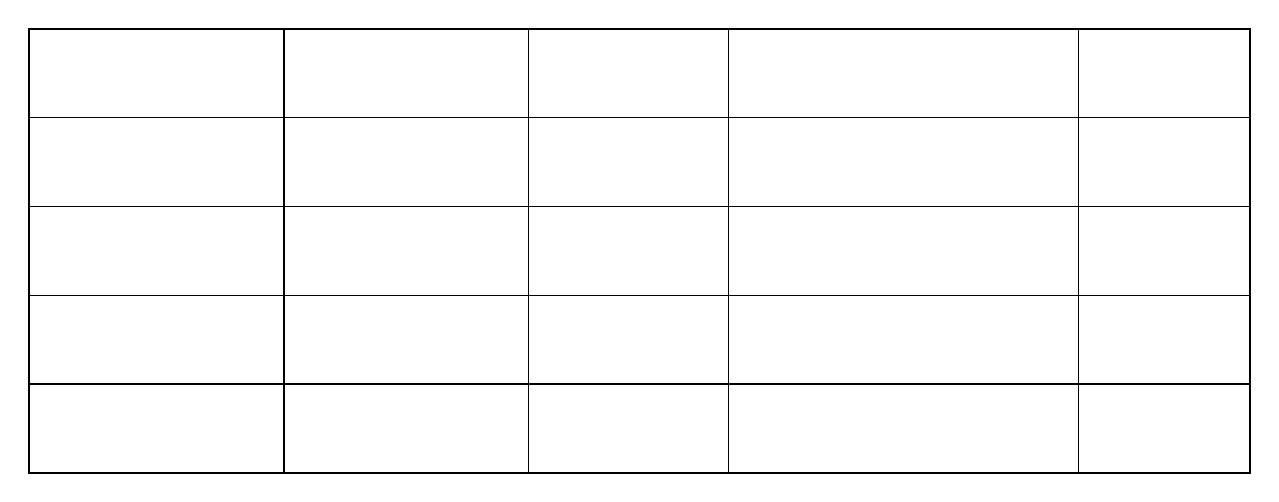
\begin{tikzpicture}[x=1bp,y=1bp]
      \draw[line width=0.7pt] (0,0) rectangle (439.6,160);
      \foreach \y in {32,64,96,128} \draw[line width=0.55pt] (0,\y) -- (439.6,\y);
      \foreach \x in {92,180,252,378} \draw[line width=0.55pt] (\x,0) -- (\x,160);
    \end{tikzpicture}}%
    \put(136,274){\makebox(0,0)[b]{\CJKfamily{coversong}\bfseries\fontsize{13pt}{16pt}\selectfont 学号}}%
    \put(226,274){\makebox(0,0)[b]{\CJKfamily{coversong}\bfseries\fontsize{13pt}{16pt}\selectfont 姓名}}%
    \put(306,274){\makebox(0,0)[b]{\CJKfamily{coversong}\bfseries\fontsize{13pt}{16pt}\selectfont 专业}}%
    \put(405,274){\makebox(0,0)[b]{\CJKfamily{coversong}\bfseries\fontsize{13pt}{16pt}\selectfont 学院}}%
    \put(497,274){\makebox(0,0)[b]{\CJKfamily{coversong}\bfseries\fontsize{13pt}{16pt}\selectfont 年级}}%
    \@cstudenttable
    \put(395,83.7){\makebox(0,0)[b]{\CJKfamily{coversong}\bfseries\fontsize{16pt}{20pt}\selectfont 时间}}%
    \put(422,83.7){\makebox(0,0)[lb]{\coverbody\fontsize{12bp}{15bp}\selectfont\@cdate}}%
  }}%
  \null
  \end{titlepage}
}
\makeatother

% Compact booktabs tables, following ACM/MICRO typographic conventions.
\newcommand{\ReportTableStyle}{%
  \renewcommand{\baselinestretch}{1}\fontsize{10.5bp}{12.6bp}\selectfont
  \renewcommand{\arraystretch}{1.08}%
  \setlength{\tabcolsep}{4.5pt}%
  \setlength{\extrarowheight}{0pt}}
\newcommand{\ReportTableHeader}[1]{{\sffamily\bfseries #1}}
\setlength{\heavyrulewidth}{0.65pt}
\setlength{\lightrulewidth}{0.35pt}
\setlength{\cmidrulewidth}{0.3pt}
\setlength{\aboverulesep}{0.45ex}
\setlength{\belowrulesep}{0.65ex}
\setlength{\defaultaddspace}{0.45ex}
\setlength{\LTpre}{5pt}
\setlength{\LTpost}{6pt}
\setlength{\textfloatsep}{11pt plus 2pt minus 2pt}
\setlength{\floatsep}{9pt plus 2pt minus 2pt}
\setlength{\intextsep}{10pt plus 2pt minus 2pt}
\renewcommand{\topfraction}{0.92}
\renewcommand{\bottomfraction}{0.85}
\renewcommand{\textfraction}{0.12}
\renewcommand{\floatpagefraction}{0.72}
\setcounter{topnumber}{4}
\setcounter{bottomnumber}{3}
\setcounter{totalnumber}{6}
\makeatletter
\setlength{\@fptop}{0pt}
\setlength{\@fpsep}{10pt plus 1fil}
\setlength{\@fpbot}{0pt plus 1fil}
\makeatother

\graphicspath{{figures/}}
\hypersetup{pdftitle={AI对话数据与智能体行为可视分析系统（知微）},pdfsubject={数据分析与可视化实践课程报告},pdfauthor={课程项目组}}
\begin{document}
	% !Mode:: "TeX:UTF-8"
\cheading{天津大学《数据分析与可视化实践》课程报告}
\ccovertitle{《数据分析与可视化实践》课程报告}
\ctitle{AI 对话数据与智能体行为可视分析系统（知微）}
\caffil{软件学院}
\csubject{软件工程}
\cgrade{2024级}
\cstudenttable{
\covermember{1}{3024232129}{李承文}{软件工程}{软件学院}{2024级}
\covermember{2}{3024244140}{仲禹潼}{软件工程}{软件学院}{2024级}
\covermember{3}{3024244438}{范文丽}{软件工程}{软件学院}{2024级}
\covermember{4}{3024244137}{赵紫怡}{软件工程}{软件学院}{2024级}
}
\cdate{2026 年 11 月 20 日}

	\frontmatter
	\pagestyle{empty}
	\makecover

	\clearpage
\begingroup
\pagestyle{empty}
\setcounter{page}{2}
\phantomsection
\pdfbookmark[0]{目录}{mulu}
\newcommand{\ReportTocRow}[3]{%
  \put(73.70,#1){\makebox(0,0)[lb]{\song\fontsize{12bp}{18bp}\selectfont
    \hbox to447.88bp{\hyperref[#2]{#3}\leaders\hbox to6bp{\hss.\hss}\hfill\pageref{#2}}}}%
}
\AddToShipoutPictureFG*{\AtPageLowerLeft{%
  \setlength{\unitlength}{1bp}%
  \put(297.64,745.92){\makebox(0,0)[b]{\song\bfseries\fontsize{18bp}{24bp}\selectfont 目录}}%
  \ReportTocRow{710}{part:purpose}{一、实验目的}
  \ReportTocRow{686}{part:team}{二、小组分工}
  \ReportTocRow{662}{part:project}{三、项目介绍}
  \ReportTocRow{638}{part:process}{四、实验过程}
  \ReportTocRow{614}{part:conclusions}{五、实验结论}
  \ReportTocRow{590}{part:experience}{六、实验体会}
  \ReportTocRow{552}{app:db}{附录 A\quad 统一数据字典与清洗质量明细}
  \ReportTocRow{528}{app:prompts}{附录 B\quad 提示策略、受测模型与实验配置}
  \ReportTocRow{504}{app:code}{附录 C\quad 关键处理与交互系统源码清单}
  \ReportTocRow{480}{app:evidence}{附录 D\quad 知微系统运行界面与多视图实测截图}
  \ReportTocRow{456}{app:environment}{附录 E\quad 运行环境、代码规模与目录映射}
  \ReportTocRow{432}{app:stats}{附录 F\quad 全维度统计结果与配对比较明细}
  \ReportTocRow{408}{app:validation}{附录 G\quad 课程评分标准对照与验收核验记录}
}}
\null
\thispagestyle{empty}
\clearpage
\endgroup


	\mainmatter\defaultfont\raggedbottom
\tolerance=2000 \emergencystretch=2em
	\renewcommand{\thelstlisting}{\arabic{chapter}-\arabic{lstlisting}}
	\makeatletter
	\fancypagestyle{plain}{
		\fancyhf{}
		\fancyhead[C]{\song\wuhao \@cheading}
		\fancyfoot[C]{\song\xiaowu ~\thepage~}
		\renewcommand{\headrulewidth}{0.5pt}
		\renewcommand{\footrulewidth}{0pt}
	}
	\makeatother
	\pagestyle{fancy}
	\setcounter{page}{3}
	\titleformat{\chapter}{\centering\fontsize{18bp}{21.6bp}\selectfont\bfseries}{\chaptername}{0pt}{}

	\chapter{实验目的}\label{part:purpose}

在日常课程学习与编写代码的实践里，我们小组成员频繁使用大语言模型辅助推导数学题、检索长篇英文文献以及调试 Python 脚本。随着使用频次增加，几个反复出现的现象引起了我们的注意：同一道数学题，有时要求模型把步骤写清楚能大幅提高正确率，有时却因为推导写得过于冗长繁琐而在输出上限处被硬生生截断；把二十篇参考资料一起塞进对话框时，模型经常漏掉夹在中间的关键句子；而在让模型修改报错代码时，单纯催促它“再仔细检查一遍”，往往不仅修不好原有漏洞，还会把原本已经写对的逻辑改坏。

面对这些零散的日常经验，《数据分析与可视化实践》课程设计题目二“AI 对话数据与智能体行为分析”为我们提供了一次用严格数据说话的机会。我们小组选择\textbf{选项 B：构建可视交互系统}，围绕上述实际痛点设计并实现了名为\textbf{“知微”}的多任务模型行为可视分析系统。之所以取名“知微”，寓意从单次 Token 消耗、单个证据段落位置和单轮报错反馈这些细微日志特征入手，观察并验证模型整体表现的变化规律。

\section{课程设计任务定位与总体目标}

对照课程设计指导书对“可视交互系统组”的考核要求，我们没有停留在把现成对话记录做成几张静态柱状图的层面，而是将工作重心放在“日志采集与脱敏清洗—同题配对统计推断—多视图联动探索系统”三个相互咬合的环节上。图~\ref{fig:roadmap} 概括了小组从最初拟定研究问题到最终完成无头浏览器回归验收的六个实施阶段。

\begin{figure}[!htbp]
\centering
\includegraphics[width=0.95\linewidth]{\detokenize{figures/diagrams/d01-roadmap.pdf}}
\caption{课程设计六阶段推进路线与阶段产出物关系}
\label{fig:roadmap}
\end{figure}

在具体实施过程中，我们为系统确立了以下四项核心实验目标：

\paragraph{规范化采集与隐私伦理保护}针对多模型、多提示策略与多轮代码执行日志建立完整的原始备份机制。所有原始 JSONL 响应文件在落盘后即做只读冻结与 SHA-256 摘要登记，一切格式转换、评分修正与字段抽取均在派生副本上完成。在对外展示与仓库交付层，严格剥离 API 密钥、本地绝对路径与账户信息，并对原始题目编号执行实验域内的单向哈希映射（\texttt{question\_key}），做到既保留同题配对分析能力，又不公开未授权的原始长对话文本。

\paragraph{异构日志整合与空值语义隔离}本项目的实验横跨数学与多选推理、多文档问答、单轮多采样代码生成以及多轮交互代码修复四类不同场景。不同场景天然带有各自的评测标尺与专有字段。我们在清洗阶段制定了 21 列统一匿名特征规范（\texttt{all\_records.csv.gz}，详细字段字典供查阅见附录~\ref{app:db}），统一布尔值、UTC 时间戳与截断判定口径，并严格区分“正常计零分（\texttt{0}）”“沙箱环境不兼容排除（\texttt{environment\_excluded}）”与“源端未记录（\texttt{null}）”，避免用草率的默认值填补污染分母。

\paragraph{尊重题目相关性的统计建模}由于同一道基准题会被多个模型、31 种提示词策略乃至 5 次重复采样反复作答，单条响应之间存在明显的题目聚类效应。如果直接把二十多万条记录当作彼此独立的伯努利试验计算标准误，置信区间会被人为压窄。因此，我们在分析阶段全面采用\emph{以独立题目为聚类单元的同题配对 Bootstrap 重采样}（默认重采样 $B=5{,}000$ 次，固定随机种子 91），并且严守描述性统计与因果解释的界限，不把特定测试集上的相关性夸大为普适定律。

\paragraph{多层次可视交互与证据溯源}为了兼顾首次浏览时的结论可读性与深入排查时的自由探索需求，我们构建了双模式前端体系：主入口（\texttt{index.html}）仅依赖浏览器原生 HTML5、CSS3 与手写 SVG 构建五球导航与五屏联动视图，老师或同学克隆仓库后只需用 Python 3.10 标准库即可一键启动；探索工作台（\texttt{explore.html} 与 \texttt{legacy.html}）则离线集成了课程指导书推荐的 ECharts、D3.js、Plotly.js 与 Vega-Lite 四类工具，支持二维散点框选、采样步进播放、分布缩放以及单题代码 Diff 抽屉溯源。

\section{核心研究问题拆解与假设边界}

\Needspace{15\baselineskip}
\begin{wrapfigure}{r}{0.47\linewidth}
\vspace{-8pt}
\centering
\includegraphics[width=\linewidth]{\detokenize{figures/diagrams/d08-research-cube.pdf}}
\caption{三维实验操控空间与五项发现映射}
\label{fig:research-cube}
\vspace{-8pt}
\end{wrapfigure}

如果把大模型本身看作参数已经固定的黑盒求解器，普通使用者在实际调用接口时真正能够主动调节的抓手主要有三个：\textbf{怎么提输出要求}（提示词组织与长度约束）、\textbf{怎么摆参考材料}（关键证据在长上下文中的位置），以及\textbf{怎么给纠错信号}（多轮交互中的测试反馈粒度）。如图~\ref{fig:research-cube} 所示，我们围绕“\emph{在不改变模型底层权重的前提下，如何组织输出表达、参考证据与执行反馈以兼顾任务质量与计算开销？}”这一总问题，设计了五项具体、可证伪的子问题，恰好对应课程指导书要求的两条低维模式、两条三维及以上交互关系和一条反常现象：

\begin{enumerate}
  \item \textbf{低维问题一（输出组织 $\to$ 质量与开销折衷）}：在数学推理任务中，从只给最终答案（\texttt{NoCoT}）切换到分步推理（\texttt{DefaultCoT}）通常会伴随数倍的 Token 增长。如果在保留分步思考的前提下加上一句温和的简洁提示（\texttt{BeConcise}），能否在数学、问答与代码任务上普遍省下可观的输出长度而不牺牲准确率？
  \item \textbf{低维问题二（作答语言模板 $\to$ 竞赛数学截断与得分）}：面对同一批英文原版数学题（如 \texttt{MATH500} 与 \texttt{GSM8K}），仅将外显作答要求改为中文（\texttt{ChineseCoT}），模型输出 Token 数、达到上限被截断的比例以及最终题目得分会发生怎样的联动变化？这种变化在不同难度题库之间是否存在明确边界？
  \item \textbf{反常现象问题（极端长度软约束 $\to$ 输出反弹与格式崩溃）}：直觉上，把提示词里的字数、词数或字母数上限压得越低，模型吐出的文本就应该越短。然而当约束收紧到“只准用 1 个词”或“只准用 10 个字母”这类极端阈值时，实际输出 Token 数是否真的单调下降？为何苛刻的格式指令会在部分模型上诱发严重的超长输出反弹甚至代码提取失败？
  \item \textbf{多维交互问题一（受测模型 $\times$ 证据位置 $\times$ 文档总数 $\to$ 问答命中率）}：在包含 10 篇或 20 篇检索文档的开放域问答中，保持问题与候选段落内容完全不变，仅把唯一包含标准答案的文档依次放到第 1 至第 20 位的不同位置上，不同模型表现出的首尾偏好（U 型曲线）深度有何差异？两代同系列模型之间的准确率优势在首段、中段和末段是否均匀分布？
  \item \textbf{多维交互问题二（受测模型 $\times$ 反馈信息粒度 $\times$ 修改轮次 $\to$ 代码强测通过率）}：当模型初稿代码未能通过测试时，连续 4 轮给予不同粒度的外部反馈——从完全不给反馈的独立重采样、无外部信号的自行检查，到仅告知通过与否、提供报错行定位诊断，再到给出单个或多个具体失败反例——模型的累积修复率、把原本正确初稿改坏的回退率以及总 Token 账单呈现怎样的三维演化规律？
\end{enumerate}

\CaseCard{方法论边界先行约定：相关性不等于内部机制因果}{
在进入后续实验分析之前，我们小组内部统一了一条贯穿全报告的写作准则：本实验采集到的全部指标均来自接口外显输入与返回文本的对照观测。例如“中文作答模板在 \texttt{MATH500} 上得分更高”，只能严格解释为\textbf{在 800 Token 输出上限条件下，中文表层表述密度更高、减少了未完结截断失败}，而绝不能凭此断言模型底层神经元“用中文思考更聪明”；同理，各提示策略在特定题集上的排序属于探索性统计证据，不能脱离采样温度与评测规则泛化为绝对优劣。}

\section{实验报告内容组织与正附分离约定}

由于整个课设周期内小组累计采集并归档了六批次共 273,186 条物理模型响应、编写了 158 个前后端与分析脚本文件（共 37,534 行代码）并产出了数十张分条件统计表，若将全部字段定义、提示词原文和分模型明细表直接堆入正文，不仅会打断分析逻辑，也会造成正文版面拥挤。

因此，本报告在编排上采取\textbf{“正文重机制推演与视觉证据、附录重规范备查与完整归档”}的结构设计。正文第~\ref{part:team} 章介绍四人分工协作机制与版本迭代过程；第~\ref{part:project} 章阐述“知微”系统的双口径数据全景、三入口界面形态与四层零依赖架构；第~\ref{part:process} 章详细展开实验设计、21 列清洗与评分器修正、五项核心统计发现、原生 SVG 与四库联动前端实现以及自动化质量回归；第~\ref{part:conclusions}、\ref{part:experience} 章总结实证启示、局限性与小组成员的真实课设收获。至于承担查阅功能的完整数据字典、31 种提示模板与模型规格、关键核心源码、原始问答与代码 Diff 案例库、多视口系统实测图集、全维度统计大表、工程目录映射及评分点核验日志，则按主题分类编排为\textbf{附录 A 至附录 H}，方便随时按需翻阅核查。

	\chapter{小组分工}\label{part:team}

\textbf{协作模式}\quad 本小组由四名同学共同完成，采用\textbf{“统一契约先行、模块并行推进、交叉测试合流”}的平权协作方式，不设组长与组员层级，所有成员均深度参与需求设计、编码实现、数据分析、系统测试与报告撰写工作。开工前，四人共同审定课程题目二的评分细则与五项研究问题，确定统一的 \texttt{snake\_case} 数据规范、21 列匿名特征 Schema 以及四份科研 JSON 快照接口格式，保证数据管道、统计脚本与前端视图之间能够端到端的无缝衔接与口径一致。

\textbf{研发推进顺序}\quad 整体研发分为四个阶段（见图~\ref{fig:roadmap}）：第一阶段完成多任务推理、文档问答与代码生成原始数据的采集、SHA-256 校验冻结及匿名化清洗脚本；第二阶段开展文档位置 9 点剖面专题与代码反馈双层隔离补充实验，并完成 5,000 次按题聚类 Bootstrap 统计重算与出版级 SVG 图稿绘制；第三阶段研发“知微”五球入口与五屏交互主系统，迁移保留完整历史探索图册，并建立基于 Python 标准库的静态构建与防漂移校验脚本；第四阶段完成 Playwright 全链路浏览器回归、无障碍审计与报告归档。

\textbf{质量与版本约定}\quad 仓库使用 Git 进行多分支协同开发，每项数据分析脚本与前端迭代均须通过 \texttt{scripts/system/check\_coursework.py} 的链接与交付物检查。任何涉及页面数值口径调整的改动，必须同步更新 \texttt{docs/} 下的口径说明与测试断言，严禁在页面代码中硬编码未经统计脚本验证的估算数据。

具体工作量与职责划分见表~\ref{tab:team-work}。

\begin{table}[!htbp]
\centering
\caption{小组成员分工与主要工作量明细}\label{tab:team-work}
\ReportTableStyle
\renewcommand{\arraystretch}{1.06}
\begin{tabularx}{\linewidth}{@{}>{\raggedright\arraybackslash}p{1.45cm}>{\raggedright\arraybackslash}p{2.35cm}>{\raggedright\arraybackslash}X@{}}
\toprule
\textbf{姓名} & \textbf{学号} & \textbf{核心职责与代码贡献} \\
\midrule
李承文 & 3024232129 & 负责研究协议与数据采集规范设计；主导文档证据位置 9 点专题实验与配对差距统计；设计代码反馈协议隔离与强保留评测模块（\texttt{experiments/code\_repair\_v2/}）；编写静态构建流水线 \texttt{build\_web\_app.py} 与科研保护校验脚本，并承担第四屏对比卡与配对统计交互逻辑开发。 \\
\addlinespace[2pt]
仲禹潼 & 3024244140 & 负责数据清洗流水线与 21 列统一匿名特征 Schema 构建（\texttt{scripts/cleaning/}）；实现聚类 Bootstrap 重算与异常缺失值审计脚本；设计“知微”五屏布局与响应式 CSS 体系（\texttt{app/styles/}）；完成历史探索图册 \texttt{explore.html} 与 \texttt{legacy.html} 的兼容整合及数据表弹窗开发。 \\
\addlinespace[2pt]
范文丽 & 3024244438 & 负责推理提示与文档问答实验的采集调度与源评分核对；主导中文作答模板与极端限长反弹异常的深度分析；开发零依赖原生 SVG 绘图引擎 \texttt{zhiwei.js} 与七大核心图版渲染模块；负责真实代码修复 Diff 案例抽取、抽屉交互组件开发及数据字典编写。 \\
\addlinespace[2pt]
赵紫怡 & 3024244137 & 负责代码生成任务的目标函数 AST 抽取与多轮修复数据规范化；独立设计与实现五球时空光晕开场入口及全键盘无障碍导航（\texttt{zhiwei-gate.js}）；主导 Playwright 浏览器双套件回归测试（\texttt{zhiwei.mjs}、\texttt{zhiwei-gate.mjs}）与单元测试编写，并负责课程报告 LaTeX 迁移排版与答辩材料校对。 \\
\bottomrule
\end{tabularx}
\end{table}

	\chapter{项目介绍}\label{part:project}

“知微”可视分析系统旨在回答大语言模型应用中的一个核心工程问题：在不改动模型底层权重的前提下，提示词的组织方式、参考证据在上下文中的排布位置，以及执行反馈的信息粒度，如何共同决定任务最终的成败与计算代价。

\begin{figure}[!htbp]
\centering
\subfigure[五球时空交互入口]{\shot[0.48\linewidth]{\detokenize{figures/screenshots/gateway.jpg}}}\hfill
\subfigure[第一屏：研究问题与任务全景]{\shot[0.48\linewidth]{\detokenize{figures/screenshots/s1-default.jpg}}}
\caption{“知微”可视交互系统首屏概览}
\label{fig:ui-overview}
\end{figure}

如图~\ref{fig:ui-overview} 所示，系统采用深空星图与“景深”光学对焦作为视觉隐喻，将原本枯燥的 26 万余条离线日志封装为可探索的数字标本。用户既可以通过五个光晕入口直达“研究问题、实验设计、数据处理、核心发现、结论与反思”五个连续交互屏，也可随时切换至保留 44 张完整科学图稿的补充探索图册。

\paragraph{工程规模与统计口径}为清晰界定工作量，图~\ref{fig:project-stats} 展示了截至提交版本的代码库物理统计。全仓包含 \textbf{158 个核心源码文件}，合计 \textbf{37,534 行代码}（其中非空行 35,695 行），涵盖前端交互脚本（10,811 行）、专项实验分析（10,386 行）、离线清洗与构建管线（7,080 行）、样式系统（5,012 行）以及自动化测试套件（3,587 行）。

\begin{figure}[!htbp]
\centering
\includegraphics[max width=\linewidth]{\detokenize{figures/diagrams/d02-project-stats.pdf}}
\caption{项目数据规模与源码工作量分布}
\label{fig:project-stats}
\end{figure}

在数据口径方面，报告与系统严格区分三组物理计数，避免混淆统计分母：
\begin{itemize}
  \item \textbf{原五项实验统一表}（\texttt{data/processed/all\_records.csv.gz}）：共 \textbf{248,586 条}物理响应，包含推理提示、文档问答、代码生成、文档位置与历史 Mini 代码修复。
  \item \textbf{代码反馈补充批次}（\texttt{code-repair-extension-free-full-20261105-3rep-v2}）：独立保存的 \textbf{24,600 条}物理响应，覆盖 164 道题 $\times$ 2 模型 $\times$ 3 份共享初稿及六种反馈处理。
  \item \textbf{主展示页面选用口径}：新版“知微”主页面采用最新完整代码反馈补充批次替换历史 Mini 批次，共呈现 \textbf{267,610 条}物理响应（$248,586 - 5,576 + 24,600$），仓库全量累计物理响应为 \textbf{273,186 条}。
\end{itemize}

下面分别从项目背景与实验矩阵、研究需求与课程对照、四层系统架构与技术选型三个方面展开介绍。

\section{项目背景与实验设计}\label{sec:project-bg}

\subsection{受测模型与三类基准任务}

为了使实验结论兼具小参数稠密模型与大参数混合专家（MoE）模型的代表性，我们选取了四款主流开源及商业接口模型进行跨任务对照（详细公开规格及来源说明见附录~\ref{app:prompts}）。在本地推理与开源部署端，选用 \texttt{Qwen2.5-7B-Instruct}（7.61B 稠密）与 \texttt{Qwen3-8B}（8.2B 稠密，并在代码反馈补充实验中显式关闭额外思考模式）；在稀疏激活大模型端，选用 \texttt{DeepSeek-V4.1-Flash-1017}（552B 骨干，预填充激活 8B / 生成激活 16B）与 \texttt{HY4 preview}（770B 骨干，每 Token 激活 49B）。

\noindent\begin{minipage}[t]{0.52\linewidth}
\vspace{0pt}
任务设置覆盖课程要求的\textbf{三类典型 AI 交互场景}：第一类为数学推理与学科选择题，采用 \texttt{GSM8K}（小学算术应用题，200 题）、\texttt{MATH500}（竞赛数学题，200 题）与 \texttt{MMLU-Pro}（多学科高难选择题，200 题）；第二类为长上下文文档问答，基于 \texttt{NQ-Open} 构建 200 道问题与 10/20 篇干扰文档组合及闭卷基线；第三类为 Python 代码生成与多轮修复，分别基于 \texttt{CodePromptEval}（清洗审核后保留 194 题）与 \texttt{HumanEval+ Mini}（164 题）开展独立采样与多轮执行反馈对照。
\end{minipage}\hfill
\begin{minipage}[t]{0.45\linewidth}
\vspace{0pt}
\centering
\captionof{table}{受测模型与任务范围概览}\label{tab:models-tasks}
\ReportTableStyle
\begin{tabularx}{\linewidth}{@{}>{\raggedright\arraybackslash}p{1.9cm} >{\raggedright\arraybackslash}X@{}}
\toprule
\textbf{维度} & \textbf{实验范围} \\
\midrule
受测模型 & Qwen2.5 7B、Qwen3 8B、DeepSeek Flash、HY4 preview \\
推理/选择 & GSM8K、MATH500、MMLU-Pro（各 200 题） \\
文档问答 & NQ-Open 200 题（10/20 篇材料 + 闭卷） \\
代码任务 & CodePromptEval 194 题；HumanEval+ 164 题 \\
\bottomrule
\end{tabularx}
\end{minipage}

\subsection{31 种提示策略与五组实验矩阵}

在推理、文档问答与代码生成实验中，我们系统构造了覆盖\textbf{回答组织、语言模板、长度预算与表达格式}四大族系的 \textbf{31 种提示策略}（完整提示文本见附录~\ref{app:prompts} 表~\ref{tab:prompts-31}）。回答组织族包含只给答案（\texttt{NoCoT}）、默认分步（\texttt{DefaultCoT}）、简洁分步（\texttt{BeConcise}）以及步数限制（\texttt{StepLimit(1/2/5)}）；语言模板族包含中文作答（\texttt{ChineseCoT}）及其四档长度组合；长度预算族涵盖词数 7 档（1 至 100 词）、字母数 4 档（10 至 500 字母）和 Token 数 4 档（10 至 500 Token）；表达格式族则包含项目符号、缩写去元音、简化语法、移除空格与纯数字算式。

针对文档上下文位置效应与代码修复闭环机制，我们进一步增设了两项专题实验：其一为\textbf{文档证据位置专题}（3,600 条响应），固定 \texttt{NoCoT} 提示与 20 篇参考文档，在保持问题完全一致的前提下，将唯一包含答案的黄金文档依次置于第 1、3、5、8、10、13、15、18、20 位，精细刻画双模型的位置剖面曲线；其二为\textbf{代码执行反馈补充实验}（24,600 条响应），在共享同一份初始代码草稿的基础上，对比独立重采样、无反馈自行检查、仅返回通过状态、错误定位诊断、单个失败反例与多个失败反例六种处理臂在四轮修改中的演化轨迹。

\section{课程设计要求落实与多入口功能协同}\label{sec:requirements}

课程设计指导书对选项 B“可视交互系统”提出了六项明确的功能闭环要求：具备清晰的分析目标、打通从日志解析到行为分类的数据管道、实现不少于 3 个核心交互视图、提供至少一种跨视图有效联动、依托系统沉淀具体案例洞察，以及交付可独立运行的代码仓库与说明文档。我们在规划系统功能时，逐条核对了指导书第 5 至第 8 页的细则（完整评分点映射表见附录~\ref{app:validation}），并在此基础上做了更扎实的工程拓展。

\begin{figure}[!htbp]
\centering
\includegraphics[width=0.92\linewidth]{\detokenize{figures/diagrams/d02-project-stats.pdf}}
\caption{“知微”系统核心规模指标与跨任务评测覆盖概览}
\label{fig:project-stats}
\end{figure}

如图~\ref{fig:project-stats} 所示，系统在任务广度、视图丰富度与交互深度三个维度均大幅超出了基准线要求：

\paragraph{四类任务与多维行为分类管道}指导书要求至少设计 2～3 类任务且总消息数不少于 150 条。本项目实际覆盖了算术与竞赛数学（\texttt{GSM8K}、\texttt{MATH500}）、多学科专业选择（\texttt{MMLU-Pro}）、多文档开放问答（\texttt{NQ-Open}）以及 Python 函数生成与多轮测试修复（\texttt{CodePromptEval}、\texttt{HumanEval+}），样本规模达二十余万条。清洗脚本不仅提取了 Token 开销、响应耗时与停止原因，还通过规则分类器与沙箱执行器自动标定了 4 类外显输出组织形态、14 类细粒度代码运行错误以及多轮修复中的“初错修复 / 初对保持 / 过度修改回退”轨迹状态。

\paragraph{主叙事七大原生图版与工作台十三类交互图种}指导书第 5 页列举了时间线、柱状/饼图/堆叠图、错误恢复路径树、散点/热力图、分组箱线图、平行坐标图与原始文本详情面板等推荐图种。我们在主站（\texttt{index.html}）第四屏手写了七幅高信息密度的原生 SVG 交互图版，聚焦回答五项核心研究问题；同时在探索工作台（\texttt{explore.html}）完整实现了模型柱图、多维雷达图、31 策略热力图、规模开销气泡图、分组环形柱图、资料位置曲线、Plotly 分组箱线图、ECharts 平行坐标图、状态饼图与堆叠图、输出形态约束矩阵、HTTP 请求时间线、重试路径前缀树以及评分分歧桑基流图共计 \textbf{13 类交互视图}，让每一种推荐图种都承载真实的分析任务而非充当摆设。

\paragraph{五重跨视图交互联动机制}为了避免“点一下按钮只换一张静态图片”的假交互，我们在系统内打通了五条真实的数据联动链路：（1）第二屏点选任意提示词单元格，实时联动右侧实际英文指令模板、实验控制条件与样本覆盖统计；（2）第三屏点选 21 列数据字典字段，同步高亮上游原始表来源、清洗转换规则与真实匿名记录切片；（3）第四屏切换模型、基准题库或测试口径时，SVG 曲线、$R^2$ 对数拟合线、右上角配对比较卡的胜负平计数与 95\% 区间同步重绘；（4）点击“真实修改案例”滑出侧边抽屉，逐轮比对 JSON 测试反馈原文与前后代码行级 Diff；（5）在探索工作台中用鼠标框选（Brush）代码开销散点区域，右侧错误构成柱状图、可评样本计数与底部匿名记录导出集合立即按框选坐标过滤同步。


\subsection{面向课堂演示与自由钻取的双轨交互动线}

在完成全部视图组件开发后，团队结合日常排查数据的真实使用习惯（文档记录于 \texttt{docs/demo-guide.md} 与 \texttt{docs/product.md}），打磨了两条互补的分析操作动线，防止用户在丰富控件中迷失方向（图~\ref{fig:demo-paths}）：

\begin{figure}[!htbp]
\centering
\subfigure[主站第二屏：默认分步基线策略卡片状态]{\shot[0.485\linewidth]{\detokenize{figures/screenshots/s2-default.jpg}}}\hfill
\subfigure[探索台引导案例：输出长度直方分布与异常入口]{\shot[0.485\linewidth]{\detokenize{figures/screenshots/explore-demo.jpg}}}
\caption{面向结构化讲解的主站策略沙盘（左）与面向异常记录排查的探索台分布入口（右）}
\label{fig:demo-paths}
\end{figure}

\paragraph{动线一：五分钟主线验证动线（宏观规律 $\to$ 配对区间 $\to$ 单题代码 Diff）}适用于首次了解本项目的读者。从首页五球门户点击进入第一屏对比不同模型在 31 策略下的基准带宽；随后滑入第二屏（图~\ref{fig:demo-paths}a）交替点击 \texttt{DefaultCoT}、\texttt{BeConcise} 与 \texttt{CharLimit(10)} 核对原始英文指令；接着在第三屏查看 21 列统一表如何将 \texttt{T149} 环境排除项置空隔离；最后进入第四屏依次切换三大题库预算拟合线、9 位置剖面与代码修复轨迹，并在右侧配对卡中将“单个失败反例”对比“自行检查”，直接拉开侧滑抽屉检视 \texttt{HumanEval/54} 一行修好集合比较的真实代码差异。

\paragraph{动线二：探索式异常归因动线（分布框选 $\to$ 错误拆解 $\to$ 匿名子集导出）}适用于追查反常样本的研究者。从探索工作台（图~\ref{fig:demo-paths}b）切入“代码生成 $\to$ 输出开销”，用鼠标在 Vega-Lite 散点图上框选“高 Token 消耗但低 Pass@1”或“极短输出低通过率”的局部点簇，观察右侧 ECharts 柱状图是否由常规断言失败突变为高达八九成的 \texttt{extraction\_error}；随后点击对应错误柱打开底层匿名评分记录表，将命中条件导出为标准 CSV 文件做离线复核。两条动线通过顶栏导航按钮双向打通，确保叙事引导与自由探索无缝切换。

\section{四层零依赖工程架构与技术选型考量}\label{sec:architecture}

在动手搭建前端之前，我们小组认真讨论过一个很现实的问题：到底要不要上 React + Vite + Node 后端服务？讨论之后我们一致投了反对票。原因很简单：课程验收时老师和助教需要在不同电脑上快速拉起项目，如果强依赖特定版本的 Node.js、复杂的 \texttt{npm install} 编译链甚至在线 CDN 脚本，一旦遇到校园网波动或环境版本冲突，整个演示就会卡在安装依赖上。

基于这一工程判断，我们将全系统划分为职责边界清晰的\textbf{四层解耦架构}（图~\ref{fig:architecture}），实现了“离线重计算在 Python、在线轻交互在原生浏览器”的运行模式。

\begin{figure}[!htbp]
\centering
\includegraphics[width=0.95\linewidth]{\detokenize{figures/diagrams/d03-architecture.pdf}}
\caption{“知微”系统四层工程架构与离线快照流转关系}
\label{fig:architecture}
\end{figure}

\noindent
\begin{minipage}[c]{0.51\linewidth}
\setlength{\parindent}{2em}\setlength{\parfillskip}{0pt plus 0.78\linewidth}
\textbf{第一层（L1）为原始字节冻结与规范数据层}。所有采集落盘的 JSONL 原始响应与评测日志存放在 \texttt{data/raw/} 下并通过 Git LFS 管理；经脱敏与类型标准化后的分实验清洗表与 21 列总表保存在 \texttt{data/processed/}，由 \texttt{SHA256SUMS.txt} 锁死字节完整性。

\textbf{第二层（L2）为离线清洗、统计推断与科研绘图层}。分布在 \texttt{scripts/} 与 \texttt{experiments/} 下的 83 个 Python 脚本（合计 17,466 行代码，源码规模分布见图~\ref{fig:loc-arch}）承担全部耗时计算，包括 AST 代码规范化、沙箱隔离执行、5,000 次按题聚类 Bootstrap 抽样以及出版级矢量图导出。

\textbf{第三层（L3）为静态构建与防漂移快照层}。构建脚本 \texttt{build\_web\_app.py} 在校验源数据与图稿 SHA-256 指纹一致后，将前端所需的统计结果打包为 \texttt{app/data/} 下仅数兆大小的匿名 JSON 快照，并为静态资源注入 12 位内容哈希后缀，彻底消除浏览器缓存旧数据的隐患。
\end{minipage}\hfill
\begin{minipage}[c]{0.465\linewidth}
\centering
\includegraphics[width=\linewidth]{\detokenize{figures/charts/c08-loc-architecture.pdf}}
\captionof{figure}{全仓库 37,534 行源码分层构成统计}
\label{fig:loc-arch}
\end{minipage}

\medskip

\textbf{第四层（L4）为零外部网络依赖的交互前端层}。启动器 \texttt{app/launch.py} 仅调用 Python 3.10+ 标准库中的 \texttt{http.server} 与 \texttt{socket} 模块即可自动完成构建检核、端口绑定与本地服务拉起。在浏览器端，主站（\texttt{index.html}）完全不加载任何第三方图表框架，直接由 \texttt{zhiwei-gate.js} 与 \texttt{zhiwei.js} 操控 DOM 与原生 SVG \texttt{viewBox}；而探索工作台（\texttt{explore.html}）所使用的 ECharts、D3 7.9.0、Vega 5.30 / Vega-Lite 5.23 与 Plotly.js 3.1.1 共 2.45\,MB 库文件均以固定版本离线内置于 \texttt{app/assets/vendor/} 目录并附许可证校验。整套系统在完全断网的环境下依然能够毫秒级响应全部交互操作。

\subsection{离线压缩载荷封装与标准库无状态服务机制}

为了让包含近九万条代码评分与十五万条问答特征的探索工作台能够在不架设后台数据库的条件下流畅筛选，我们在 L3 构建层与 L4 浏览器运行时之间设计了\textbf{“Gzip 分片静态特征包 + 预编译全局运行时脚本”}的轻量传输方案：

\begin{itemize}
  \item \textbf{冷热数据分层加载}：首屏与主叙事五屏所需的汇总统计、置信区间与精选案例体积控制在数百 KB 以内（如 \texttt{research-charts.json} 仅 93\,KB、\texttt{code-feedback-extension.json} 仅 212\,KB），页面打开瞬间即可完成解析与首帧渲染；而体量较大的逐样本匿名特征明细（如 1.85\,MB 的 \texttt{features.json.gz} 与 1.18\,MB 的 \texttt{code-features.json.gz}）仅在用户切入探索工作台打开箱线图或记录抽屉时按需异步拉取解压。
  \item \textbf{零构建工具链的纯标准库启动器}：入口脚本 \texttt{app/launch.py} 不依赖 Flask、FastAPI 或任何第三方 Web 容器。启动时，它先调用内部构建器核验 \texttt{app/dist/} 快照指纹，随后通过标准库 \texttt{http.server.ThreadingHTTPServer} 在本地环回地址 \texttt{127.0.0.1} 上挂载多线程静态文件服务，自动配置 \texttt{.wasm}、\texttt{.woff2} 与 \texttt{.svg} 的标准 MIME 类型并处理端口冲突提示，真正做到克隆即运行。
\end{itemize}


	\chapter{实验过程}\label{part:process}

本章顺着系统的全链路工程顺序，依次记录多任务数据采集与伦理脱敏、数据清洗与 21 列统一结构化、聚类统计与五项核心发现的实证分析、“知微”交互可视化系统研发、静态快照契约构建、全链路自动化回归测试，以及研发中攻克的四项关键技术难点。正文仅保留高信息密度的核心对照表与典型代表图表，其余全量字段字典、31 种提示策略原文、全分组统计明细与多视口截图均归档于附录 A 至附录 G。

\section{多任务实验方案设计与原始日志采集}\label{sec:collection}

\subsection{四大任务场景与六批次对照矩阵}

为了避免只在单一简单题集上得出片面结论，我们在采集方案设计阶段选取了知识形态、输入长度与评判方式截然不同的四类代表性任务，累计形成六个冻结实验批次：

\paragraph{数学推理与多学科选择（74,400 条物理响应）}选取小学算术应用题 \texttt{GSM8K}、英文竞赛数学 \texttt{MATH500} 与多学科高阶选择题 \texttt{MMLU-Pro} 三个基准，每个基准固定抽取 200 道独立题目，分别在 \texttt{Qwen2.5-7B}、\texttt{Qwen3-8B}、\texttt{DeepSeek Flash} 与 \texttt{HY4 preview} 四个模型上遍历全部 31 种提示词策略（$4\times 3\times 200\times 31 = 74{,}400$ 条）。采集脚本固定单次生成上限以观察不同提示长度下的自然截断现象，并完整记录接口返回的输入/输出 Token 数、结束原因（\texttt{finish\_reason}）与源判分结果。

\paragraph{多文档开放域问答与九位置精细扫描（74,800 + 3,600 条）}基于自然问题数据集 \texttt{NQ-Open} 的 200 道事实型问题，构造两阶段上下文位置实验。第一阶段基线实验同时涵盖无参考材料的闭卷控制组（每模型 200 条），以及供给 10 篇或 20 篇检索段落并将唯一含答案文档（Gold Document）置于首部、中部或尾部的全策略对照，在两个 Qwen 模型上共采集 74,800 条响应；第二阶段专题实验（\texttt{configs/document\_positions.json}）为精细刻画“中间迷失”曲线形状，固定使用简洁直接的 \texttt{NoCoT} 指令与 20 篇参考文档，将含答案文档依次放入第 \textbf{1、3、5、8、10、13、15、18、20} 共 9 个精确序号位置（$2\times 200\times 9 = 3{,}600$ 条），从而排除了提示词格式噪声对位置效应的干扰。

\paragraph{单轮多采样代码生成（90,210 条）}采用经过可执行性筛选的 \texttt{CodePromptEval} 基准中 194 道 Python 函数任务，横跨“无外部依赖独立函数”“仅依赖标准库”“依赖第三方包”与“跨文件工程级依赖”四个复杂度层级。在 \texttt{DeepSeek Flash}、\texttt{Qwen2.5-7B} 与 \texttt{Qwen3-8B} 三个模型上遍历 31 种任务适配后的提示策略，并对每个“模型 $\times$ 题目 $\times$ 提示”组合执行 5 次低温度独立采样（$3\times 194\times 31\times 5 = 90{,}210$ 条），专门用于检验重复采样饱和度与提示词多样性增益。

\paragraph{多轮代码执行反馈修复（5,576 条基线 + 24,600 条双层隔离补充）}在早期完成 5,576 条多轮修复基线探索后，团队针对 \texttt{HumanEval+ Mini} 的全部 164 道 Python 编程题重新设计了严格受控的补充采集协议（图~\ref{fig:repair-protocol}）。我们先为每个模型（\texttt{Qwen2.5-7B} 与 \texttt{Qwen3-8B}，显式关闭 Qwen3 额外思考模式以拉平推理预算）每道题生成 3 份低温独立初稿（\texttt{temperature=0.2}，共 $2\times 164\times 3 = 984$ 份物理共享初稿），随后从每一份相同的初稿分叉出六种反馈处理臂，各自连续推进 4 轮生成（$984 + 984\times 6\times 4 = 24{,}600$ 条唯一物理响应）。

\begin{figure}[!htbp]
\centering
\includegraphics[width=0.95\linewidth]{\detokenize{figures/diagrams/d05-repair-protocol.pdf}}
\caption{多轮代码修复补充实验的共享初稿分叉与公开/保留测试物理隔离协议}
\label{fig:repair-protocol}
\end{figure}

\subsection{31 种提示词策略族系与六臂反馈梯度}

为了让实验对比具有清晰的结构层次，我们将 31 种单轮提示词归纳为四个对照族系（完整英文原文模板与参数见附录~\ref{app:prompts}）：（1）\textbf{回答组织族}（6 种），包括 \texttt{NoCoT}、\texttt{DefaultCoT}、\texttt{BeConcise} 以及限制推理步数的 \texttt{StepLimit(1/2/5)}；（2）\textbf{语言模板族}（5 种），包括切换中文作答的 \texttt{ChineseCoT} 及其带字数上限的四个变体 \texttt{ChineseCoT(10/50/100/500)}；（3）\textbf{长度预算族}（15 种），按词数 \texttt{WordLimit(1..100)}、字母数 \texttt{CharLimit(10..500)} 和词元数 \texttt{TokenLimit(10..500)} 设置由松到紧的软约束梯度；（4）\textbf{表达格式族}（5 种），包括仅列要点 \texttt{BulletPoints}、缩写去元音 \texttt{AbbreviateWords}、忽略语法 \texttt{NoProperGrammar}、去空格换行 \texttt{NoSpaces} 与仅用数字算式 \texttt{OnlyNumbers}。在代码生成任务中，我们将格式与长度约束限定在代码围栏之外的解释文字上，避免直接破坏 Python 关键字语法。

而在多轮代码修复补充实验中，六种处理臂按外部执行信息量由零到强严格递增：（1）\textbf{独立重采样（\texttt{resample}）}：每轮只重新传入原题，不保留历史代码与报错；（2）\textbf{自行检查（\texttt{self\_review}）}：传入上一轮候选代码并要求复查修正，但不提供任何测试结果；（3）\textbf{仅通过状态（\texttt{pass\_fail}）}：仅告知公开诊断测试为 \texttt{PASS} 或 \texttt{FAIL}；（4）\textbf{错误定位诊断（\texttt{diagnostic}）}：提供首个报错的异常类型、行号与调用栈摘要，隐去具体测试输入与期望输出；（5）\textbf{单个失败反例（\texttt{counterexample}）}：给出首个失败公开用例的输入、期望输出与实际输出；（6）\textbf{多个失败反例（\texttt{multi\_counterexample}）}：最多给出前 3 个失败公开用例及测试通过计数摘要。

\subsection{原始制品只读冻结与伦理脱敏措施}

采集脚本运行过程中，每条 API 请求均以追加写模式实时落盘至 \texttt{data/raw/} 下的 JSONL 文件，并同步记录配置哈希 \texttt{config\_sha256}。全部跑批结束后，我们对 405 余份原始数据制品生成校验清单并设为只读，后续任何清洗重算脚本均被禁止改写原始目录（验证测试会检查 \texttt{api\_calls == 0}）。

在伦理与隐私合规方面，本实验全部基于公开学术基准题库与模型接口生成，不涉及真实人类受试者的私人聊天记录。清洗导出阶段，脚本自动剥离环境变量中的 API Key、服务商内部请求头及本地机器路径，并通过作用域哈希函数 \texttt{sha256((direction + "|" + question\_id).encode())[:24]} 生成 24 位十六进制伪匿名题号 \texttt{question\_key}。前端公开部署包仅携带数值统计特征与少量人工脱敏核查后的教学示例片段，严格遵循课程指导书第 3 页的伦理要求。

\subsection{异步并发采集调度、断点续采与异常重试日志治理}

二十七万余条模型接口调用并非一蹴而就，在跨越数天的批量采集过程中，云端 API 偶发的速率限制（HTTP 429）、网关瞬时超时（HTTP 502/504）以及本地网络抖动都是必须正面处理的工程常态。为此，我们在 \texttt{scripts/acquisition/} 与 \texttt{experiments/code\_repair\_v2/} 的采集器中内置了三项容错保障：

\paragraph{进程级互斥锁与幂等断点续采}每次启动跑批脚本时，程序首先在实验工作目录创建 \texttt{.collection.lock} 文件锁，防止误开两个终端并发覆盖同一输出流。重连恢复时，采集器先扫描已落盘 JSONL 文件构建已完成任务键集合 \texttt{completed\_keys = \{(model, task\_id, prompt\_id, sample\_id)\}}，自动跳过已成功获取完整响应的单元，确保中途断网重跑不会产生重复计费或脏行。

\paragraph{指数退避重试与完整 HTTP 状态轨迹留存}遇到可恢复的服务端限流或瞬断时，调度器按带随机抖动的指数退避间隔发起有限次重试，并将每一次尝试的起止时间戳、HTTP 状态码与累计尝试次数（\texttt{attempt\_count}）原样写入日志。这些真实保存下来的通信元数据没有在清洗时被丢弃，而是直接转化为了探索工作台中的“请求时间线”与“重试路径前缀树”两类行为视图。

\paragraph{评测计划前置哈希锁定}在代码修复补充实验中，采集器在发出第一条请求前先将全部 164 道题目列表、模型参数、随机种子与六臂名称固化写入 \texttt{plan.json} 并计算 \texttt{config\_sha256}；后续每一条物理响应与沙箱评测回执都必须携带匹配的 \texttt{config\_sha256}，否则离线分析器将拒绝合并，从源头杜绝了中途临时改配置混跑数据的隐患。

\section{异构日志清洗、21 列特征归并与评分器迭代修正}\label{sec:cleaning}

\subsection{异构源日志解析与 21 列统一匿名 Schema}

把六批次原始日志摆在一起时，我们面临的第一个脏活就是格式对齐：推理实验保存的是带源评分与复核标记的宽表，文档问答包含 46 列 HTTP 重试与四套匹配指标，代码生成是逐样本 JSONL 加独立沙箱评测文件，而代码修复还存在父子轮次引用链。为此，我们在 \texttt{scripts/cleaning/} 下搭建了分阶段清洗归并流水线（图~\ref{fig:data-pipeline}）。

\begin{figure}[!htbp]
\centering
\includegraphics[width=0.95\linewidth]{\detokenize{figures/diagrams/d04-data-pipeline.pdf}}
\caption{从异构原始 JSONL 日志到 21 列统一匿名特征表与静态快照的清洗流程}
\label{fig:data-pipeline}
\end{figure}

\Needspace{15\baselineskip}
\begin{wrapfigure}{r}{0.46\linewidth}
\vspace{-8pt}
\centering
\includegraphics[width=\linewidth]{\detokenize{figures/charts/c07-missingness-audit.pdf}}
\caption{21 列统一特征在五类实验中的非空完备率审计}
\label{fig:missing-audit}
\vspace{-10pt}
\end{wrapfigure}

归并脚本 \texttt{build\_unified\_features.py} 将所有物理响应映射为结构统一的 21 列压缩表 \texttt{all\_records.csv.gz}，同时导出记录血缘表 \texttt{record\_lineage.csv.gz}。在这套 Schema 中，我们坚持了三条清洗铁律：

一是\textbf{物理去重记账}。在代码修复任务里，六个反馈臂的第 0 轮共享同一份初稿生成结果；归并脚本仅将该物理初稿写入一次，通过 \texttt{parent\_record\_key} 维护分叉拓扑，绝不把 6,560 行逻辑展开视图重复混入物理响应总账单。

二是\textbf{原生指标分列命名、严禁跨任务混算}。每条记录以 \texttt{metric\_name} 明确标注其原生主指标（如推理为 \texttt{source\_score}、文档问答为 \texttt{final\_answer\_contains}、代码生成为 \texttt{test\_pass}、代码修复为 \texttt{base\_and\_heldout\_pass}），从表结构上阻止把代码单元测试通过率与开放问答字符串包含率混成一个毫无物理意义的“总分”。

三是\textbf{严格区分空值（\texttt{null}）与零分（\texttt{0}）}。如图~\ref{fig:missing-audit} 的全量缺失率审计所示，诸如推理与代码生成历史归档未记录请求时间戳（完备率 0\%）、文档问答闭卷控制组无证据位置（400 条记录空置，完备率 99.5\%）、代码修复初稿无父节点（1,640 条空置，完备率 70.6\%）以及代码生成沙箱环境排除（465 条记录的 \texttt{metric\_value} 置为 \texttt{null}，完备率 99.5\%），全部具有明确的实验结构成因（完整 105 项审计明细见附录~\ref{app:db}）。清洗脚本对空值统一输出空单元格并在校验器中禁止零值填充，防止样本分母失真。

\subsection{输出形态规则分类与代码执行错误编码}

为了支撑行为模式分布分析，脚本 \texttt{classify\_and\_audit.py} 对模型回复文本与执行结果做了两级确定性分类。在文本组织层面，利用正则表达式识别显式步骤标记（如 \texttt{Step 1}、\texttt{第一步}）、项目符号列表、无标记多行段落与单行短答四类可见输出形态（\texttt{output\_style}），并与请求状态、长度截断标志组合成四类互斥结果状态（请求失败、长度截断、答案未解析、正常判分）。

在代码任务层面，评测器根据语法树解析与沙箱运行回执，将失败响应细分为断言失败（\texttt{AssertionError}，代表代码可运行但逻辑不符）、代码提取失败（\texttt{extraction\_error}，代表回复中未能解析出有效函数）、类型错误（\texttt{TypeError}）、名称与导入错误（\texttt{NameError} / \texttt{ImportError}）、语法缩进错误、超时与内存受限等 14 个细类，为后续诊断“提示词究竟改坏了算法逻辑还是破坏了输出格式”提供了直接依据。

\subsection{两次关键清洗踩坑与评分器修正纪实}

在检查第一轮初步统计表时，我们没有急于画图，而是抽样核对了数百条原始报错日志，结果抓出了两处足以改变实验结论的系统性测量偏差，并逐一完成了工程修正：

\Needspace{15\baselineskip}
\begin{wrapfigure}{l}{0.45\linewidth}
\vspace{-6pt}
\centering
\includegraphics[width=\linewidth]{\detokenize{figures/diagrams/d10-ast-v2-pipeline.pdf}}
\caption{代码生成 \texttt{target-function-ast-v2} 规范化抽取与沙箱预检流程}
\label{fig:ast-v2}
\vspace{-8pt}
\end{wrapfigure}

\paragraph{修正一：重写 AST-v2 消除类方法缩进误报}在 \texttt{CodePromptEval} 第一轮自动测试跑完后，我们惊讶地看到大量肉眼完全正确的 Python 代码被判成了 \texttt{IndentationError} 或安全违规。顺着日志追查源代码才发现两个隐藏陷阱：其一，基准中不少目标函数其实是类里面的实例方法，官方参考代码本身带有 4 格类内缩进，初版评测脚本直接把切片喂给 \texttt{ast.parse} 自然当场报缩进错；其二，模型习惯在函数上方写 \texttt{import re}、\texttt{from typing import Optional} 或辅助小函数，若原样按 4 格缩进塞回类体内部，导入语句就会变成类属性定义，而旧版沙箱白名单又错误拦截了部分标准库导入。

针对这一问题，我们在 \texttt{evaluate\_responses.py} 中彻底重写了 \texttt{target-function-ast-v2} 规范化器（流程见图~\ref{fig:ast-v2}，核心代码见附录~\ref{app:code}）：先调用 \texttt{textwrap.dedent} 剥离外层缩进并解析语法树，精准定位同名目标函数；再把模型写在顶层的 \texttt{Import}、常量赋值与辅助函数节点安全内迁至目标函数文档字符串之后；同时从官方参考函数自动继承参数类型注解、返回值注解与装饰器，防止测试模板因缺少 \texttt{List} 等类型导入报假错。接着，我们让官方参考实现在完全相同的无网络、仅允许临时目录写入的沙箱策略下做前置预检，发现编号为 \texttt{T149} 的题目连官方标准答案都会因沙箱外路径访问而失败。我们将这 $3\times 31\times 5 = 465$ 条记录如实标记为 \texttt{environment\_excluded=true} 移出正确率分母，使其余 193 道共同可评题（89,745 条记录）的通过率回归真实水平。

\begin{figure}[!htbp]
\centering
\subfigure[四套问答判分规则下的命中率分歧]{\includegraphics[width=0.485\linewidth]{\detokenize{figures/charts/base-05_document_qa_metric_sensitivity.pdf}}}\hfill
\subfigure[不同提示格式引发的截断与漏判分布]{\includegraphics[width=0.485\linewidth]{\detokenize{figures/charts/base-06_document_qa_format_truncation.pdf}}}
\caption{多文档问答任务中判分规则敏感性诊断与格式截断交叉分析}
\label{fig:docqa-metric-sens}
\end{figure}

\paragraph{修正二：多文档问答四标尺并存揭示“答对但判错”}在清洗 74,800 条文档问答记录时，我们也遇到了类似的测量难题：原论文常用的首行匹配（\texttt{paper\_firstline}）要求模型把答案放在第一行，但当叠加了 \texttt{DefaultCoT}（先分步思考）提示词后，模型自然会把推理过程写在前面、把最终答案放在末尾；反之，若采用末尾行严格精确匹配（\texttt{strict\_final\_em}），模型只要多写一个句号或冠词就会被判零分。统计诊断表显示，在 \texttt{Qwen2.5-7B} 与 \texttt{Qwen3-8B} 各自的 37,200 条全策略回答中，全文实际已包含标准答案但被严格末行精确匹配判负的记录分别高达 \textbf{8,624 条}与 \textbf{11,415 条}！如图~\ref{fig:docqa-metric-sens} 所示，我们在清洗表中完整保留了全部四套判分列，选定对分步推理与简答均更公平的末段标准化包含率（\texttt{final\_contains}）作为主分析标尺，并在探索工作台中专门设计了“评分分歧桑基流图”供直观比对。

\subsection{高风险样本分层抽样复核与多轮血缘图消歧}

除了自动化清洗与 AST-v2 评分修正外，我们还针对自动规则最容易出偏差的灰色地带补充了两项人工与结构审计工作：

\paragraph{170 条高风险边界样本分层复核抽样}在数学推理与多选问答的 74,400 条记录中，当模型回答带有复杂单位（如 \texttt{2516\_8}、\texttt{\$203}）、分数等价形式或没有按标准格式在末行写出 \texttt{Answer:} 时，纯正则提取可能发生漏判。为此，脚本 \texttt{classify\_and\_audit.py} 按“长度截断、首末行提取不一致、无显式标记多行输出”等风险层分层抽取了 \textbf{170 条代表性样本}导出至 \texttt{reports/baseline/scoring-review-sample.csv}，同时将此前已人工逐条核实的 139 条争议答案判分结论固化进复核覆盖表（在清洗表的 \texttt{grading\_status} 列明确区分“已判分”与“已按保存的逐条复核结论判分”），绝不暗中手工涂改原始分数。

\paragraph{多轮代码修复的物理节点与逻辑视图严格分离}在整理多轮修复数据时，一个极易把样本数算糊涂的陷阱是“共享初稿复用”。由于每一道题的同一份第 0 轮初稿同时作为 6 种反馈策略的共同起点，如果按“6 个策略 $\times$ 5 个版本（R0–R4）”直接展开成平面宽表（\texttt{features.csv}），每份初稿就会在表里重复出现 6 次。我们在清洗规范中明确将此类展开表界定为\emph{仅供画逐轮轨迹折线使用的逻辑视图}；而在计算总物理响应条数（24,600 条）与生成统一格式压缩表（\texttt{unified-records.csv.gz}）时，严格按 \texttt{physical\_record\_id} 去重，确保第 0 轮共享初稿只计入一次，并通过 \texttt{shared\_seed\_id} 与 \texttt{parent\_id} 无损还原整棵分叉修改树。


\paragraph{311 条跨条件极端反差样本自动归档}为了支撑前端点击异常点时能够秒级调出具有代表性的同题反差证据，我们编写了 \texttt{scripts/system/export\_special\_records.py}，在离线阶段扫描配对清洗表，自动筛出“默认分步因超长截断得 0 分而温和简洁分步拿满分”“宽松 100 字母上限顺利答对而极限 10 字母上限反弹截断”“首行匹配判错但末段包含判对”等 \textbf{311 条典型跨条件交叉异常记录}，经脱敏核验后压缩存入 \texttt{app/data/special-records.json.gz}（145\,KB），使每一个统计反常点背后都有真实可查的单题记录支撑。

\section{统计推断建模与五项核心实验发现剖析}\label{sec:analysis}

\subsection{按题聚类配对 Bootstrap 与多任务统计量定义}

\Needspace{15\baselineskip}
\begin{wrapfigure}{r}{0.47\linewidth}
\vspace{-8pt}
\centering
\includegraphics[width=\linewidth]{\detokenize{figures/diagrams/d11-bootstrap-cluster.pdf}}
\caption{按独立题簇有放回配对 Bootstrap 推断流程}
\label{fig:bootstrap-flow}
\vspace{-8pt}
\end{wrapfigure}

在本项目采集的数据结构中，每道基准题往往挂载着多达数十条关联响应（例如推理题库中同一道题对应 4 个模型 $\times$ 31 种提示共 124 条回答，代码修复中同一道题对应 2 个模型 $\times$ 3 份初稿 $\times$ 6 个反馈臂的多轮轨迹）。刚开始写统计脚本时，我们曾对比过“按单条响应做普通二项正态近似”和“按题目聚类重采样”的区间宽度，发现前者因为把同一道难题上的重复失败当成了独立证据，算出的标准误比真实情况偏小近一半，极易制造虚假的“统计显著”。

为此，我们在 \texttt{scripts/analysis/} 与 \texttt{experiments/code\_repair\_v2/src/analyze.py} 中全面统一为\textbf{以独立题目为聚类单元的配对 Bootstrap 重采样框架}（流程见图~\ref{fig:bootstrap-flow}）。设某项对比包含 $Q$ 道共同可评独立题簇 $\{1,\dots,Q\}$，在第 $b$ 次重采样（总次数固定为 $B=5{,}000$，随机种子固定为 \texttt{seed=91}）中，算法从题号集合中有放回地抽取容量为 $Q$ 的题簇索引序列 $I_b = (q_1,\dots,q_Q)$，并同步取出每个被抽中题簇在条件 $A$ 与条件 $B$ 下的成功计数 $(s_{A,q}, s_{B,q})$ 与分母计数 $(n_{A,q}, n_{B,q})$，按簇内计数之和的比值计算配对差值：
\begin{equation}
\Delta_b = \frac{\sum_{q \in I_b} s_{A,q}}{\sum_{q \in I_b} n_{A,q}} - \frac{\sum_{q \in I_b} s_{B,q}}{\sum_{q \in I_b} n_{B,q}}.
\end{equation}
将 $\{\Delta_1,\dots,\Delta_{5000}\}$ 升序排列后，直接取第 2.5\% 与第 97.5\% 分位数作为 95\% 探索性置信区间，并同步统计同题或同初稿层面的“赢 / 输 / 平”绝对频数。在代码修复实验里，尽管 164 道题乘以 3 份独立初稿共有 492 份候选程序轨迹，重采样依然严格在 164 个独立题簇上执行，绝不把 492 份程序冒充为 492 道独立题目。

针对单轮五次独立采样的代码生成任务，假设某“模型 $\times$ 题目 $\times$ 提示”单元在 $n$ 次有效可评运行中有 $c$ 次通过全部断言，我们采用 Chen 等提出的无偏组合估计量计算至少命中一次的概率，避免直接取前 $k$ 次样本带来的顺序抽样方差：
\begin{equation}
\text{Pass@}k = 1 - \frac{\binom{n - c}{k}}{\binom{n}{k}}, \qquad k \in \{1, 3, 5\}.
\end{equation}
而在衡量推理任务中提示策略的平均输出长度 $\overline{T}_p$ 与准确率 $S_p$ 的宏观关系时，我们对非极端异常策略拟合对数预算回归模型 $\widetilde{S}_p = \beta_0 + \beta_1 \ln(\overline{T}_p)$，并以样本内决定系数 $R^2$ 评估对数律在不同模型架构上的适用程度（全部回归参数详见附录~\ref{app:stats}）。

\subsection{低维发现一：输出预算的对数边际递减与温和简洁分步效应}

在数学推理任务上，我们验证的第一个核心问题是“让模型少说废话，会不会把准确率一起砍掉”。先看最直观的 \texttt{Qwen2.5-7B / GSM8K}（200 道同题配对）基线：如果强制要求模型只输出最终答案而不做任何解释（\texttt{NoCoT}），平均每次回答只花 6.5 个 Token，但正确率惨跌至 \textbf{22.0\%}；一旦切换为常规分步推理（\texttt{DefaultCoT}），正确率立即跃升至 \textbf{91.5\%}（同题配对提升 $+69.5$ 个百分点，95\% 区间 $[63.0, 76.0]$），代价是平均输出暴涨近 36 倍达到 236.7 Token。

\begin{figure}[!htbp]
\centering
\includegraphics[width=0.96\linewidth]{\detokenize{figures/charts/story-01-budget-and-concise.pdf}}
\caption{推理预算的对数收益曲线与跨任务温和简洁分步（\texttt{BeConcise}）对照概览}
\label{fig:story-concise}
\end{figure}

把全部 31 种策略放在“平均输出 Token—准确率”平面上观察（图~\ref{fig:story-concise} 左半幅），可以清楚看到明显的\textbf{对数边际收益递减规律}：对于稠密架构的 \texttt{Qwen2.5-7B}，在 \texttt{GSM8K}、\texttt{MATH500} 与 \texttt{MMLU-Pro} 三个题库上，平均输出长度的对数能解释全 31 策略得分方差的 \textbf{91.2\%、74.7\% 与 83.5\%}（若只看 7 档词数上限，\texttt{GSM8K} 上的 $R^2$ 高达 0.939）；从几十个 Token 增至一百五十个 Token 时正确率爬升极快，但超过两百个 Token 后曲线迅速进入平坦高原区，继续拉长篇幅几乎不再产生额外正确率。

\noindent
\begin{minipage}[c]{0.50\linewidth}
\setlength{\parindent}{2em}\setlength{\parfillskip}{0pt plus 0.78\linewidth}
既然超过临界预算后的冗长叙述属于“无效膨胀”，我们在保留分步思考指令的同时加上温和简洁约束（\texttt{BeConcise}：\emph{Think step by step before answering, but be concise.}）。图~\ref{fig:concise-compact} 将横跨数学推理/选择题（12 组）、多文档问答（2 组）和代码生成（3 组）共计 \textbf{17 个模型 $\times$ 任务组合}汇总在同一张象限图中：所有数据点全部落在右侧（\textbf{17/17 全组实现输出缩短}，Token 节省幅度介于 11.4\% 至 57.5\% 之间），同时有 \textbf{15/17 组落在零线及上方阴影区}，即准确率持平甚至不降反升！

为什么缩短输出反而能在竞赛数学上提分（如 \texttt{Qwen3 / MATH500} 节省 20.9\% Token 的同时准确率净升 $+11.5\text{ pp}$，\texttt{DeepSeek / MATH500} 净升 $+7.0\text{ pp}$）？翻查具体配对样本后我们找到了原因：在固定单次输出上限的场景下，温和简洁提示删掉了反复自我怀疑与二次验算的枝蔓，让模型在预算耗尽前顺利写出最终答案。
\end{minipage}\hfill
\begin{minipage}[c]{0.475\linewidth}
\centering
\includegraphics[width=\linewidth]{\detokenize{figures/charts/c02-concise-17-compact.pdf}}
\captionof{figure}{17 组模型$\times$任务下 \texttt{BeConcise} 的压缩率与得分变化象限分布}
\label{fig:concise-compact}
\end{minipage}

\CaseCard{同题配对实证（MATH500 二进制转八进制题：记录 Z012672 vs.\ Z012872）}{
题目要求将二进制数 $10101001110_2$ 转化为八进制数（标准答案 \texttt{2516}）。在 \texttt{DefaultCoT} 下，\texttt{DeepSeek Flash} 其实在第 2 步就已经按三位一组正确算出了 $010_2=2, 101_2=5, 001_2=1, 110_2=6 \Rightarrow 2516_8$；但它紧接着自发开启了“Step 3: Double-check by converting binary to decimal”，逐项展开 $2^{10}+2^8+\dots$，结果在算到第 800 个 Token 时触发长度硬截断（\texttt{finish\_reason=length}），因未输出末行答案被判 \textbf{0 分}。而同一模型在 \texttt{BeConcise} 下仅用 \textbf{89 个 Token} 干净利落地完成分组换算并给出 \texttt{Answer: 2516}，顺利拿到满分（完整原文对照见附录~\ref{app:cases}）。}

\subsection{低维发现二：中文作答模板在 MATH500 上的防截断提分与适用边界}

我们在梳理语言模板族数据时注意到了第二个有趣的低维规律：当面对全英文题干的竞赛数学题库 \texttt{MATH500} 时，仅仅把提示词从英文默认分步改成一句简短的中文作答指令（\texttt{ChineseCoT}：\emph{Respond in Chinese.}），四个受测模型的平均输出 Token 全部下降，而且其中三个模型的最终得分出现了肉眼可见的跃升。

\noindent
\begin{minipage}[c]{0.475\linewidth}
\centering
\includegraphics[width=\linewidth]{\detokenize{figures/charts/c03-chinese-3tasks.pdf}}
\captionof{figure}{切换中文作答模板在三个基准题库上的准确率变化与 Token 压缩对比}
\label{fig:chinese-3tasks}
\end{minipage}\hfill
\begin{minipage}[c]{0.495\linewidth}
\setlength{\parindent}{2em}\setlength{\parfillskip}{0pt plus 0.78\linewidth}
对照图~\ref{fig:chinese-3tasks} 的实测数值可以看到，在 \texttt{MATH500} 上，\texttt{Qwen3-8B} 的准确率从 58.0\% 大幅升至 \textbf{69.5\%}（$+11.5\text{ pp}$，Token 节省 19.5\%），\texttt{HY4 preview} 从 68.5\% 升至 \textbf{74.0\%}（$+5.5\text{ pp}$，节省 19.5\%），\texttt{Qwen2.5-7B} 从 68.0\% 升至 \textbf{70.5\%}（$+2.5\text{ pp}$，节省 33.3\%），而原本得分最高的 \texttt{DeepSeek Flash} 则稳定维持在 75.0\% 附近并同步节省 4.4\% 的输出词元开销。

为了搞清楚多出来的分数从哪来，我们编写了 \texttt{math-completion-recovery.csv} 专项追踪脚本，把那些“英文答错、中文答对”的救援题单拎出来检查。结果非常一致：在 \texttt{HY4} 被中文模板救回来的 21 道题里，有 \textbf{20 道}原本在英文分步下死于 800 Token 长度截断；\texttt{Qwen2.5} 救回的 19 题中有 \textbf{13 题}原为截断（整组截断率更是从 22.0\% 骤降到 \textbf{2.5\%}）；\texttt{Qwen3} 救回的 30 题中也有 \textbf{18 题}原为截断。
\end{minipage}

\medskip

换句话说，中文数学表述在现有分词器下具有更高的单 Token 语义承载密度（比如英文写“Therefore, substituting $x = 8k + 5$ into the second inequality gives”需要十几个词元，中文写“代入第二个不等式得”只需寥寥数个词元）。在长推导容易撞上输出天花板的难题上，这种紧凑性帮模型抢在截断前完成了收尾（如附录~\ref{app:cases} 收录的 \texttt{Z049851/Z054851} 分装硬币同余题）。

\paragraph{严格界定任务适用边界}如果只看 \texttt{MATH500}，很容易草率得出“用中文提问全面优于英文”的片面结论；但只要结合图~\ref{fig:chinese-3tasks} 中的橙色条形（\texttt{GSM8K}）一对比就能保持清醒：虽然全部 12 组“四模型 $\times$ 三题库”对照在切换中文后都节省了 4.4\%～48.7\% 的 Token，但在步骤简单、英文截断率本就接近 0\% 的小学算术题 \texttt{GSM8K} 上，四个模型切换中文后没有任何“防截断红利”可吃，反而因跨语种题干理解转换损耗出现了 \textbf{$-0.5$ 至 $-4.5\text{ pp}$} 的轻微掉分。这再次印证了跨多题库交叉验证的必要性。

\subsection{反常现象剖析：极端长度与格式软约束引发的 Token 反弹与提取崩溃}

既然温和地提示“简洁一点”能省 Token 保质量，那么把紧箍咒越念越紧——比如强令模型“只准用 10 个词，甚至只准用 1 个词”或者“最多只准用 10 个英文字母”——输出长度是不是就会一路压到最低？实验结果给出了一个截然相反的反常现象。

\begin{figure}[!htbp]
\centering
\includegraphics[width=0.95\linewidth]{\detokenize{figures/charts/story-02-extreme-limit-rebound.pdf}}
\caption{收紧词数上限（左）与字母数上限（右）时出现的输出 Token 反常暴涨现象}
\label{fig:extreme-rebound}
\end{figure}

如图~\ref{fig:extreme-rebound} 所示，当词数要求从 100 词逐步收紧到 10 词时，各模型的平均输出长度确实如预期般顺畅下降；但当上限从 \texttt{WordLimit(10)} 推向极端的 \texttt{WordLimit(1)} 时，12 个“模型 $\times$ 题库”分组中有 \textbf{9 组平均输出 Token 不仅没减，反而大幅反弹上升}！同样地，当字母上限从 \texttt{CharLimit(100)} 压紧到 \texttt{CharLimit(10)} 时，同样有 \textbf{9/12 组出现剧烈的长度逆向反弹}。同时，图~\ref{fig:limit-compliance-errors}(a) 对 \texttt{TokenLimit(10/50/100/500)} 的实测均值追踪也表明，自然语言提示词属于软约束而非解码器硬截断：在 \texttt{TokenLimit(10)} 下，各模型在 \texttt{MATH500} 上的超标率普遍超过 95\%，模型根本无法凭文本指令精确数准自己的子词切分数目。

\begin{figure}[!htbp]
\centering
\subfigure[MATH500 上名义 Token 约束与实测均值偏离]{\includegraphics[width=0.48\linewidth]{\detokenize{figures/charts/c04-token-compliance.pdf}}}\hfill
\subfigure[代码生成任务中三模型的细粒度错误构成对比]{\includegraphics[width=0.495\linewidth]{\detokenize{figures/charts/cg-05-error-cats.pdf}}}
\caption{软长度约束偏离诊断与极端提示对代码生成错误类型的冲击}
\label{fig:limit-compliance-errors}
\end{figure}

最典型的反弹样本出现在 \texttt{DeepSeek Flash / MATH500} 上：从 \texttt{CharLimit(100)} 收紧至 \texttt{CharLimit(10)} 时，该组平均输出从 102.0 Token 暴涨五倍多达到 \textbf{520.6 Token}，正确率则从 83.5\% 断崖式跌至 \textbf{38.0\%}。我们调出单题记录 \texttt{Z015404} 终于看清了反弹的微观机制：

\CaseCard{异常反弹微观溯源（记录 Z015404：求 196 的正因数个数，CharLimit(10)）}{
模型在前三行仅用不到 40 个 Token 就完美完成了质因数分解：$196 = 2^2\times 7^2 \Rightarrow (2+1)(2+1) = 9$。然而看到“Only use 10 letters for your answer”后，模型陷入了荒诞的自我纠结：“Nine 只有 4 个字母，不够 10 个字母怎么办？写成 NINENINENI？还是找一个表示 9 的 10 字母英文单词？Ennead 是 6 个字母，Novenary 是 8 个字母……”它就这样反复数着字母个数自言自语了整整 \textbf{760 多 Token}，直到耗尽 801 Token 被强制截断，最终连本来早就求出的数字 \texttt{9} 都没来得及输出！}

在代码生成任务（\texttt{CodePromptEval}）中，极端格式与简省指令同样引发了严重的次生灾害。结合图~\ref{fig:limit-compliance-errors}(b) 的错误分类统计可以看到，除了常规的断言逻辑失败（占 26.6\%～36.3\%）之外，\textbf{代码提取错误（\texttt{extraction\_error}）}在两个 Qwen 模型上分别占到了 12.31\% 和 \textbf{22.08\%}。一旦施加破坏排版的极端格式提示，如 \texttt{Qwen2.5} 在 \texttt{NoProperGrammar} 下的函数提取失败率飙升至 \textbf{94.5\%}，\texttt{Qwen3} 在 \texttt{OnlyNumbers} 下提取失败率达 \textbf{78.7\%}，甚至在 \texttt{NoCoT} 下也有 \textbf{44.0\%} 的回答因为模型机械照搬“不给任何额外包装”而漏写 Markdown 代码块围栏（见附录~\ref{app:cases} 记录 \texttt{Y080666}），导致本可运行的代码直接折戟在解析阶段。

\subsection{多维交互一：受测模型 $\times$ 证据位置 $\times$ 文档规模的问答命中规律}

进入三维及以上多变量分析，我们先考察开放域多文档问答（\texttt{NQ-Open}）中“模型能力、文档总篇数与核心证据排布位置”三者的交互效应。首先以闭卷零文档控制组锚定底线：在不提供任何检索段落、纯靠预训练参数记忆盲答时，\texttt{Qwen2.5-7B} 与 \texttt{Qwen3-8B} 的标准化包含命中率分别为 \textbf{29.0\%} 与 \textbf{27.5\%}，两者处于几乎相同的记忆起跑线。

\begin{figure}[!htbp]
\centering
\includegraphics[width=0.95\linewidth]{\detokenize{figures/charts/docpos-profile.pdf}}
\caption{20 篇参考文档下两代 Qwen 模型在 9 个精细证据位置的命中率剖面与 95\% 区间}
\label{fig:docpos-9}
\end{figure}

当引入外部参考文档并将文档总数从 10 篇扩充至 20 篇时（图~\ref{fig:docqa-pos-multi}a），两个模型在中间段落的命中率均因无关干扰文档增多而明显下滑，呈现出经典的“首尾高、中间低”U 型注意力衰减特征；而在图~\ref{fig:docqa-pos-multi}(b) 的 31 策略 $\times$ 位置热力矩阵中也能看到，无论外层套用何种提示词，中段位置（Middle）始终是一条贯穿全局的浅色低谷带。

\begin{figure}[!htbp]
\centering
\subfigure[10 篇与 20 篇文档在首/中/尾位置的衰减对比]{\includegraphics[width=0.49\linewidth]{\detokenize{figures/charts/c05-docqa-expansion.pdf}}}\hfill
\subfigure[跨提示词策略与证据位置的命中率热力分布]{\includegraphics[width=0.48\linewidth]{\detokenize{figures/charts/lim-05-heatmap.pdf}}}
\caption{参考文档规模扩张效应与跨策略位置敏感性全貌}
\label{fig:docqa-pos-multi}
\end{figure}

更关键的三维交互出现在固定 \texttt{NoCoT} 与 20 篇文档的 9 位置精细扫描实验中（图~\ref{fig:docpos-9}）：\textbf{模型升级带来的收益并不是一条平行上移的直线，而是高度依赖证据所处的位置！}具体而言：
\begin{itemize}
  \item \textbf{首部锚定区（第 1 位）}：\texttt{Qwen3-8B} 命中率高达 \textbf{71.0\%}，而 \texttt{Qwen2.5-7B} 仅为 54.5\%，两代模型的同题配对差距达到惊人的 \textbf{$+16.50$ 个百分点}；
  \item \textbf{中段抗干扰区（第 3 至第 18 位）}：随着黄金证据滑入长上下文腹地，\texttt{Qwen3-8B} 虽也回落至 58.5\%～61.5\% 平台，但始终稳定压制滑落至 50.0\%～52.5\% 的 \texttt{Qwen2.5-7B}，保持着 \textbf{$+7.50$ 至 $+11.00\text{ pp}$} 的中段检索优势（例如题目 \texttt{C007} 询问“谁拥有最多的游击手金手套奖”，当正确文档排在第 1 位或第 20 位时模型准确答出 \texttt{Ozzie Smith}，而埋在第 10 位时则被相邻干扰段落误导答成了 \texttt{Omar Vizquel}）；
  \item \textbf{末尾近因恢复区（第 20 位）}：\texttt{Qwen2.5-7B} 借助紧邻问题末尾的近因效应回弹至 \textbf{56.5\%}，而 \texttt{Qwen3-8B} 停留在 \textbf{59.0\%}，两模型的差距骤然收窄至 \textbf{$+2.50\text{ pp}$}（置信区间横跨零点）。
\end{itemize}

这一非线性交互说明，如果评测只看文档放在末尾时的表现，我们会误以为两代模型相差无几；唯有拉通整条位置剖面，才能看清新一代模型真正的突破点在于\emph{首段强聚焦与中段抗稀释能力}。

\subsection{多维交互二：代码独立采样饱和与“模型 $\times$ 反馈粒度 $\times$ 轮次”修复轨迹}

最后一项多维分析聚焦于 AI 辅助编程中最核心的实践抉择：当模型第一次写出的代码没跑通测试时，究竟应该多抽几次盲盒（独立重采样），让模型自己反思检查，还是必须接入真实沙箱把报错或反例喂回去？我们先从 \texttt{CodePromptEval} 的 89,745 条单轮可评记录考察无反馈独立采样的天花板（图~\ref{fig:codegen-passk-div}）。

\begin{figure}[!htbp]
\centering
\subfigure[三模型无偏 Pass@1 / Pass@3 / Pass@5 饱和趋势]{\includegraphics[width=0.48\linewidth]{\detokenize{figures/charts/cg-01-model-passk.pdf}}}\hfill
\subfigure[跨提示多样性增益与工程级外部依赖落差]{\includegraphics[width=0.495\linewidth]{\detokenize{figures/charts/c06-code-diversity-dep.pdf}}}
\caption{单轮代码生成的重复采样边际递减、提示多样性效应与依赖复杂度鸿沟}
\label{fig:codegen-passk-div}
\end{figure}

如图~\ref{fig:codegen-passk-div}(a) 所示，单靠低温独立重复采样虽然能把 \texttt{DeepSeek Flash} 的通过率从 \texttt{Pass@1} 的 30.22\% 推升至 \texttt{Pass@3} 的 33.73\%，但到了第 5 次调用（\texttt{Pass@5} = 34.97\%），单次新增解决率已萎缩到仅剩 \textbf{$+0.47\text{ pp}$}（两个 Qwen 模型第 5 次边际增益同样不足 $0.8\text{ pp}$），原因是在同一提示词下模型极易连续五次掉进同一个语法或API误用坑里。有趣的是，图~\ref{fig:codegen-passk-div}(b) 进一步揭示：在完全相同的预期输出 Token 预算下，\textbf{换用 5 种不同提示词各采一次}全面优于同一提示连采 5 次（全池提升 $+2.67$ 至 $+7.15\text{ pp}$，即便剔除极端提示、仅在常规分步池内轮换也稳定净赚 $+1.80$ 至 $+3.99\text{ pp}$）；而一旦任务从独立纯函数跨越到涉及仓库外部类的工程级依赖，三模型的 \texttt{Pass@1} 更会集体暴跌 \textbf{28.95 至 48.86 个百分点}。这充分说明，没有外部执行信号介入的“蒙眼重抽”很快就会触顶。

\begin{figure}[!htbp]
\centering
\subfigure[六种反馈臂在公开诊断集上的逐轮轨迹]{\includegraphics[width=0.485\linewidth]{\detokenize{figures/charts/repair-02-public-trajectories.pdf}}}\hfill
\subfigure[严格配对队列在强保留集上的真实轨迹]{\includegraphics[width=0.485\linewidth]{\detokenize{figures/charts/repair-06-strong-trajectories.pdf}}}
\caption{多轮代码修复补充实验中公开诊断通过率（左）与完整强保留测试通过率（右）的四轮演化对比}
\label{fig:repair-trajectories}
\end{figure}

当我们进入 \texttt{HumanEval+ Mini} 的 24,600 条双层隔离多轮修复实验（每模型 164 题 $\times$ 3 份共享初稿 = 492 份程序轨迹），“模型 $\times$ 反馈粒度 $\times$ 修改轮次”的三维交互图景便清晰浮现出来（图~\ref{fig:repair-trajectories} 与图~\ref{fig:repair-mech}）：

\begin{figure}[!htbp]
\centering
\subfigure[初稿错误修复数与初稿正确回退数拆解]{\includegraphics[width=0.485\linewidth]{\detokenize{figures/charts/repair-03-repair-regression.pdf}}}\hfill
\subfigure[累计输出 Token 成本与终稿强测准确率折衷]{\includegraphics[width=0.485\linewidth]{\detokenize{figures/charts/repair-04-cost-quality.pdf}}}
\caption{六种反馈策略的“正向修复 vs.\ 反向改坏”机制拆解与计算开销帕累托前沿}
\label{fig:repair-mech}
\end{figure}

\paragraph{第一，无执行证据的“自行检查”存在改坏正确初稿的回退风险}从共享初稿出发（\texttt{Qwen2.5} 初稿强测通过 382/492 = 77.6\%，\texttt{Qwen3} 初稿通过 370/492 = 75.2\%），若不跑测试、仅让模型连续四轮“自行检查（\texttt{self\_review}）”，\texttt{Qwen3} 在耗费 4,431 平均总 Token 后终稿仅从 370 份微增至 376 份（净修好 9 份初错，却把 3 份原本正确的代码改坏了）；\texttt{Qwen2.5} 更是在自检过程中把 \textbf{8/382 份原本已经通过强测的正确初稿改出了新 Bug}（例如 \texttt{HumanEval/50} 凯撒移位解码题，初稿完全正确，自检轮次却画蛇添足加上 \texttt{if ch.isalpha()} 过滤，导致含非字母字符的隐藏用例直接挂掉）。

\paragraph{第二，反馈粒度对不同模型呈现非对称放大效应，单反例性价比最高}只要接入沙箱给出最简的 \texttt{PASS/FAIL} 状态，两个模型的回退数立刻被压制到接近零（\texttt{Qwen3} 在所有带真实执行状态的四个策略下实现 \textbf{0/370 零回退}！），因为模型收到 \texttt{PASS} 后便不再乱改已跑通的实现。继续加码反馈信息量时，两模型的响应斜率显著分化：\texttt{Qwen2.5} 从“错误定位诊断”（401/492）升级到“单个失败反例”（401/492）已基本饱和；而 \texttt{Qwen3-8B} 则表现出极强的反例吸收能力——从自行检查的 376/492，一路阶梯式攀升至仅状态的 395/492、定位诊断的 409/492、\textbf{单个失败反例的 418/492（85.0\%，初错修复率高达 48/122 = 39.3\%，配对净胜自检 $+8.54\text{ pp}$，95\% 区间 $[4.88, 12.60]$）}，以及多个反例的 421/492（85.6\%）。不过，对比图~\ref{fig:repair-mech}(b) 的横轴开销可见，“多个失败反例”比“单个反例”多消耗了约 15.6\%～17.0\% 的总 Token，终稿强测差值却仅有 $+0.61\text{ pp}$（\texttt{Qwen3}）与 $-0.41\text{ pp}$（\texttt{Qwen2.5}），置信区间均跨过零点，说明\textbf{提供首个最小失败反例已抓住绝大部分有效纠错信号}。

\paragraph{第三，公开诊断曲线与强保留测试曲线之间横亘着真实的“过拟合盲区”}对比图~\ref{fig:repair-trajectories}(a) 与 (b) 的纵轴刻度可以发现，到第 4 轮结束时，反例反馈在公开诊断集上的表观通过率已逼近甚至超过 92\%，但在未曾曝光的 \texttt{HumanEval+} 强保留集上实际停留在 81.5\%～85.6\% 之间，存在约 \textbf{7～10 个百分点的系统性落差}。我们在核查 \texttt{HumanEval/22}（筛选列表中的整数）等样本时看到，候选代码用 \texttt{isinstance(x, int)} 轻松跑通了不含布尔值的所有公开测试并收到 \texttt{PASS}，模型遂停止修改；但在 Python 中 \texttt{bool} 是 \texttt{int} 的子类（\texttt{isinstance(True, int) == True}），一遇到强保留集里的布尔边界用例便立刻露馅。这一发现也反向证明了我们坚持双层隔离评测、绝不拿公开测试通过率充当终稿成绩的必要性。

\subsection{扩展对比一：步数显式约束与格式压力策略的跨任务分化}

除了温和简洁与极端字词上限外，31 种提示策略中还包含限制显式步骤数的 \texttt{StepLimit(1/2/5)} 以及五种强格式改写指令（\texttt{BulletPoints}、\texttt{OnlyNumbers}、\texttt{AbbreviateWords}、\texttt{NoProperGrammar}、\texttt{NoSpaces}）。把这些策略横向拉通对比（图~\ref{fig:step-format-atlas}），能够更清楚地看到\textbf{“结构化压缩”与“破坏性压缩”的分水岭}：

\begin{figure}[!htbp]
\centering
\subfigure[跨模型与题库的对数预算拟合优度差异]{\shot[0.485\linewidth]{\detokenize{figures/atlas/budget-fit-comparison.pdf}}}\hfill
\subfigure[极限紧缩相对宽松档位的输出长度反弹倍率]{\shot[0.485\linewidth]{\detokenize{figures/atlas/limits-rebound-ratios.pdf}}}
\caption{不同模型架构下预算对数律的拟合优度分化（左）与极限软约束反弹倍率（右）}
\label{fig:step-format-atlas}
\end{figure}

\begin{itemize}
  \item \textbf{步数梯度（\texttt{StepLimit}）呈现平滑可控的阶段性恢复}：以 \texttt{Qwen2.5-7B} 为例，从零解释 \texttt{NoCoT}（\texttt{GSM8K} 得分 22.0\%）放宽到仅允许 1 步概括的 \texttt{StepLimit(1)}，得分便迅速恢复至 \textbf{81.5\%}，放宽至 \texttt{StepLimit(2)} 与 \texttt{StepLimit(5)} 后进一步升至 \textbf{84.5\%} 与 \textbf{85.5\%}（\texttt{MATH500} 上同样由 34.0\% 稳步升至 59.0\%、64.5\% 与 68.5\%）。相比定死的词数或字母数上限，按逻辑步数约束不会强迫模型数字符个数，因此从未触发输出反弹。
  \item \textbf{纯算式与要点化（\texttt{OnlyNumbers} / \texttt{BulletPoints}）存在显著的任务耦合性}：在纯算术题 \texttt{GSM8K} 上，要求“只写数字与算式”使 \texttt{DeepSeek Flash} 用极短篇幅依然保持高分，\texttt{Qwen2.5} 也拿到 70.0\%；但一旦迁移到需要自然语言实体匹配的文档问答或需要合法函数头部的代码生成任务，\texttt{OnlyNumbers} 便会直接抹除必要的文本或语法骨架（如 \texttt{Qwen3} 代码提取失败率飙升至 78.7\%）。而 \texttt{NoSpaces}（禁用空格与换行）则在所有任务上造成分词器切分退化与 Python 缩进语法全面瘫痪，属于典型的负向干扰指令。
  \item \textbf{高起点稀疏模型在难题上可能出现负向对数斜率}：图~\ref{fig:step-format-atlas}(a) 还揭示了一个值得注意的架构差异——不同于 \texttt{Qwen2.5} 的高正斜率对数曲线，\texttt{HY4 preview} 在 \texttt{MATH500} 上的对数回归斜率为负值（$\beta_1 = -12.26$），原因是该模型在短中预算提示下本身已具备较强解题能力，而在长篇幅提示下反而更容易撞上 800 Token 截断天花板，拉低了高 Token 区间的平均得分。
\end{itemize}

\subsection{扩展对比二：代码修复“首次公开通过即早停”测算与缺失逻辑边界}

在实际部署编程智能体时，工程师很少会让模型机械跑满固定 4 轮修改，更常见的做法是\textbf{“一旦当前代码跑通公开测试，立即停止后续调用（Stop-on-Public-Pass）”}。为了定量评估这一工程策略的得失，我们对已保存的完整五版轨迹执行了严格的离线早停回放测算（图~\ref{fig:stop-budget-atlas}）。

\begin{figure}[!htbp]
\centering
\subfigure[Qwen3 固定跑满五版与首次公开通过即早停的开销对比]{\shot[0.485\linewidth]{\detokenize{figures/atlas/feedback-stop-budget.pdf}}}\hfill
\subfigure[早期多轮修复实验中 Qwen3 各轮次增益对照]{\shot[0.485\linewidth]{\detokenize{figures/atlas/feedback-rounds-qwen3.pdf}}}
\caption{代码修复轨迹的早停回放 Token 节省测算（左）与轮次边际收益递减规律（右）}
\label{fig:stop-budget-atlas}
\end{figure}

如图~\ref{fig:stop-budget-atlas}(a) 所示，由于超过七成的共享初稿在第 0 轮即已通过公开测试，启用“首次公开通过即保留”规则可以将 \texttt{Qwen3-8B} 在具体失败反例策略下的题均累计输入输出开销从跑满五版的 \textbf{4,880.3 Token 大幅压缩至 1,334.0 Token（节省高达 72.7\%）}，在仅通过状态与自行检查策略下同样可削减逾七成的 API 账单。

与此同时，我们在补充实验分析器中严格守住了另一条方法论红线：当某次实验需要评估未完整跑完或未在中间轮测量隐藏强测试的策略时，\textbf{绝对不能拿终稿强测结果去填补中间轮的未知值，也不能把基础设施超时未测当成 0 分}。我们在 \texttt{planned-endpoint-bounds.csv} 中专门引入了 Manski 风格的缺失敏感性逻辑上下界——分别计算“假设所有未知记录全部失败（Worst-Case）”与“假设所有未知记录全部通过（Best-Case）”两个极端边界下的通过率区间。在本仓库最终交付的 \texttt{code-repair-extension-free-full-20261105-3rep-v2} 批次中，全部 164 道题 $\times$ 3 初稿 = 492 份程序均完成了 100\% 强保留验证（\texttt{unknown = 0}），上下界完全收敛重合为精确点估计，证明最终报告结论不存在任何缺失样本偏差。


\subsection{扩展对比三：代码修复首轮错误状态转移与真实案例图版剖析}

为了进一步弄清外部反馈究竟修好了哪一类 Bug，我们基于 \texttt{error-transitions.csv} 对第 0 轮共享初稿进入第 1 轮修改时的四态转移矩阵（模块加载失败 \texttt{load}、运行期异常 \texttt{runtime}、输出不匹配 \texttt{output\_mismatch} 与测试通过 \texttt{pass}）做了细粒度追踪，并结合衍生图册中的错误谱系与单题演化图版（图~\ref{fig:atlas-err-case}）交叉印证：

\begin{figure}[!htbp]
\centering
\subfigure[代码生成与修复的细粒度错误类别谱系]{\shot[0.485\linewidth]{\detokenize{figures/atlas/feedback-code-errors.pdf}}}\hfill
\subfigure[真实代码案例跨轮次修改与测试状态演进]{\shot[0.485\linewidth]{\detokenize{figures/atlas/feedback-real-code-case.pdf}}}
\caption{代码任务错误类别构成全景（左）与单题跨轮次反馈纠偏演化示意（右）}
\label{fig:atlas-err-case}
\end{figure}

从状态转移频数（完整数字见附录~\ref{app:stats} 表~\ref{tab:app-f-transitions}）可以观察到两条清晰的微观规律：其一，\textbf{语法与加载期崩溃（\texttt{load}）最容易在首轮被外部诊断一次性清除}。例如在 \texttt{Qwen2.5-7B} 的 12 份初稿加载失败程序中，一旦给出“单个失败反例”或“定位诊断”，第 1 轮就有 \textbf{8/12 份（66.7\%）}直接跨越中间错误态一步跃迁至 \texttt{pass}；而在“自行检查”下模型看不见报错行，仍有半数卡在原加载异常中。其二，\textbf{深层逻辑偏差（\texttt{output\_mismatch}）是决定模型修复上限的分水岭}。面对初稿占比最高的输出不匹配错误，仅告知 \texttt{FAIL} 状态很难帮模型猜出遗漏了哪种边界条件，唯有注入具体输入输出反例对，才能推动 \texttt{Qwen3-8B} 在四轮内稳步消化近四成的初错存量。

\section{“知微”交互可视化系统设计与实现}\label{sec:visualization}

“知微”可视化系统定位为服务科研复核与课程演示的可探索交互界面。系统代码集中在 \texttt{app/} 目录下，核心由入口控制器 \texttt{zhiwei-gate.js}（259 行）、主图版与联动引擎 \texttt{zhiwei.js}（1,760 行）、多套响应式样式表（5,012 行）以及面向全量图库的探索页面 \texttt{explore.html} / \texttt{legacy.html} 构成。

\subsection{五球时空入口与全键盘无障碍导航}

为了克服传统仪表盘开屏信息过载的问题，系统首屏设计为“光学对焦五球时空门”（\texttt{zhiwei-gate.js}）。页面初始化时利用 HTML5 Canvas 绘制低饱和度星野粒子背景，并在中央光学标尺环（动态生成 96 条放射刻度 \texttt{zw-optic-ticks}）周围排布对应“研究问题、实验设计、数据处理、核心发现、结论与反思”的五个交互光球。

\noindent\begin{minipage}[t]{0.48\linewidth}
\vspace{0pt}
\textbf{渐进式动效与无障碍兼容}\quad 开场动画持续 3,400\,ms，随后自动激活全部光球控件；用户可随时点击“跳过开场”或重播。当检测到操作系统开启 \texttt{prefers-reduced-motion: reduce} 时，脚本自动跳过粒子飞入与光球轨迹过渡，直接呈现稳定态入口；同时完整支持方向键（上下左右）、\texttt{Home/End} 切换光球焦点、\texttt{Enter} 进入章节及 \texttt{Escape} 返回入口，浏览器前进/后退与 URL Hash 深链接（如 \texttt{\#s4}）均可精确恢复状态。
\end{minipage}\hfill
\begin{minipage}[t]{0.49\linewidth}
\vspace{0pt}
\centering
\includegraphics[width=\linewidth]{\detokenize{figures/diagrams/d06-frontend-modules.pdf}}
\captionof{figure}{前端交互控制器与四类联动状态流}
\label{fig:frontend-modules}
\end{minipage}

\subsection{视觉编码规范与三页七图版核心设计}

在核心发现页（第四屏 \texttt{\#s4}），我们摒弃了 ECharts 等黑盒模板，全部使用 \texttt{zhiwei.js} 编写原生 SVG 渲染器。为防止多图切换时产生认知混淆，全站严格固化以下视觉编码规则：
\begin{itemize}
  \item \textbf{模型通道色标固定}：\texttt{Qwen2.5 7B} 恒定使用紫罗兰（\texttt{\#6749e2}）、\texttt{Qwen3 8B} 使用暖橙（\texttt{\#e07227}）、\texttt{DeepSeek Flash} 使用翡翠绿（\texttt{\#32a67d}）、\texttt{HY4 preview} 使用洋红（\texttt{\#bc1e72}）。
  \item \textbf{双编码冗余传达}：任何得分增减与状态变化基于 \texttt{oklch(L, C, hue)} 感知均匀空间计算顺序列紫与紫—橙发散色，并同时使用\textbf{颜色映射 + 文本符号 / 误差线}及 \texttt{fitText} 标签防溢出裁剪机制传达；例如发散差值采用紫—橙发散色带并附带带正负号的百分点数值（pp）。
  \item \textbf{坐标截断与口径透明}：所有截取局部 Y 轴的图版（如文档位置剖面或代码修复轨迹）均在读图说明弹窗（\texttt{i} 按钮）与脚标中显式声明坐标范围、独立题目分母及置信区间计算口径。
\end{itemize}

\begin{figure}[!htbp]
\centering
\subfigure[总体规律页（图版 I–IV）]{\shot[0.48\linewidth]{\detokenize{figures/screenshots/s4-a.jpg}}}\hfill
\subfigure[专项页：中文模板与文档位置（图版 V–VI）]{\shot[0.48\linewidth]{\detokenize{figures/screenshots/s4-b.jpg}}}
\caption{第四屏前两页核心发现全景交互视图}
\label{fig:s4-ab}
\end{figure}

如图~\ref{fig:s4-ab} 所示，第四屏通过顶部三个无障碍 \texttt{role="tab"} 选项卡组织七个核心图版：\textbf{第一页（图版 I–IV）}呈现对数预算曲线（支持切换 GSM8K/MATH500/MMLU-Pro 并动态绘制 $R^2$ 拟合虚线）、模型基准排序对比、17 组简洁分步气泡散点以及极端限长反弹柱状图；\textbf{第二页（图版 V–VI）}并列呈现四模型中文作答箭头/得分变化矩阵与 20 篇文档九位置误差带剖面；\textbf{第三页（图版 VII）}则聚焦多轮代码修复，如图~\ref{fig:s4-c-drawer} 所示，左侧绘制六策略五版本折线轨迹（支持切换“公开诊断/完整强测”与模型），右上放置可实时选定对照双方的“配对比较卡”，右下嵌入“终稿区间 / 修复与回退 / Token 代价 / 初稿错误”四子页签容器。

\begin{figure}[!htbp]
\centering
\subfigure[专项代码修复页（图版 VII 与配对比较卡）]{\shot[0.48\linewidth]{\detokenize{figures/screenshots/s4-c.jpg}}}\hfill
\subfigure[侧边真实修改案例抽屉（代码 Diff 与反馈原文）]{\shot[0.48\linewidth]{\detokenize{figures/screenshots/case-drawer.jpg}}}
\caption{代码修复多维度交互分析与真实案例溯源抽屉}
\label{fig:s4-c-drawer}
\end{figure}

\subsection{精细微交互与探索图册兼容}

除了主图切换外，系统还在每个图版右上角内置了\textbf{“说明（i）”展开面板}与\textbf{“查看数据表”模态框}，允许评阅人随时调出底层精确数值列表（支持键盘 ESC 关闭与焦点回归）；点击“真实修改案例”按钮则会从右侧滑出 \texttt{\#case-drawer} 抽屉，逐轮展示反馈 JSON 载荷与前后 Python 代码行级 Diff 高亮。

\begin{figure}[!htbp]
\centering
\subfigure[结构化数据表弹窗]{\shot[0.32\linewidth]{\detokenize{figures/screenshots/table-dialog.jpg}}}\hfill
\subfigure[探索分析工作台（explore.html）]{\shot[0.32\linewidth]{\detokenize{figures/screenshots/explore-overview.jpg}}}\hfill
\subfigure[44 张完整科学图册（legacy.html）]{\shot[0.32\linewidth]{\detokenize{figures/screenshots/atlas.jpg}}}
\caption{弹窗数据查阅与历史完整探索图册入口}
\label{fig:dialogs-explore}
\end{figure}

同时，对于希望查看所有 44 张衍生科学图稿（包含错误恢复路径图、行为时间线、分组箱线图与平行坐标图等课程指导书提及图种）的用户，系统通过第五屏导航及路由 \texttt{explore.html}、\texttt{legacy.html?chapter=atlas} 完整保留了浅色高对比度科研图册工作台（图~\ref{fig:dialogs-explore}），兼顾叙事体验与全量查阅需求。

\section{静态快照防漂移契约与工程难点攻关}\label{sec:contracts-challenges}

\subsection{构建管线 SHA-256 指纹互锁与防漂移机制}

在多人同时迭代统计脚本、科学图稿与前端页面的几周里，最容易出纰漏的地方就是“上游重跑了某个 CSV，下游网页数据包却忘了同步更新”。为了把这种人为疏忽彻底拦在构建阶段，我们在 \texttt{scripts/system/build\_web\_app.py} 与 \texttt{check\_web\_snapshot.py} 中建立了一套严格的哈希互锁契约：

\begin{itemize}
  \item \textbf{图证同源强校验}：每次执行构建或运行 \texttt{python3 app/launch.py} 时，脚本都会重新计算 \texttt{code-evidence.json} 与压缩特征包 \texttt{code-features.json.gz} 的字节级 SHA-256 摘要，并与 \texttt{figure-metadata.json} 中记录的源指纹逐一比对；一旦发现图稿与数据包不属于同一次快照生成，构建器当场抛出异常终止打包，绝不允许新旧口径混装上线。
  \item \textbf{静态产物内容寻址防缓存}：所有拷贝至 \texttt{app/dist/} 运行目录的样式表与脚本均自动追加由文件内容计算出的 12 位版本查询串（如 \texttt{?v=64c2ad0fc74d}），同时对内置的四大前端可视化库核验许可证与包哈希，确保本地离线打开时不会读到陈旧的浏览器磁盘缓存。
  \item \textbf{科研资产保护白名单}：脚本 \texttt{check\_reconstruction.py} 对仓库内 37 幅核心主题 SVG、12 份数据源清单及总计 \textbf{1,100 项已验收科研文件指纹}建立只读保护监控，确保美化界面交互时不会无意篡改任何一条实验曲线的坐标数值。
\end{itemize}

\section{全链路自动化测试与可复现性验证}\label{sec:validation}

高质量的可视化系统不仅需要图表美观，更必须经得起数值复算、链接完整、多视口排版及无障碍规范的严格检验。为此，团队构建了覆盖“静态交付 $\to$ 科研指纹 $\to$ 协议单测 $\to$ 真实浏览器交互”的四层自动化质量保证体系（图~\ref{fig:qa-matrix}）。

\begin{figure}[!htbp]
\centering
\includegraphics[max width=\linewidth]{\detokenize{figures/diagrams/d07-qa-matrix.pdf}}
\caption{四层自动化质量保证与回归验证矩阵}
\label{fig:qa-matrix}
\end{figure}

\paragraph{结构链接与科研保护核验}脚本 \texttt{scripts/system/check\_coursework.py} 使用纯标准库扫描全仓 15 份核心 Markdown 文档，在最新一次执行中自动校验了 \textbf{185 处本地相对链接与锚点}，确认课程原文与网页受保护副本的 SHA-256 完全一致，且不存在失效链接或残留副本。另一侧的 \texttt{scripts/system/check\_reconstruction.py} 则针对 37 个主题 SVG、12 份数据源清单以及 1,100 项受保护科研文件指纹执行完整性校验（在未拉取大体积 LFS 原始归档时，脚本仍能清晰区分“离线快照完整”与“LFS 未水化”状态）。

\paragraph{代码修复协议单元测试}在 \texttt{tests/test\_repair\_v2\_analysis.py}（25 项测试）与 \texttt{tests/test\_repair\_v2\_protocol.py}（8 项测试）中，我们针对代码修复补充实验编写了 33 项隔离单元测试，涵盖“防隐藏答案泄漏到反馈构造器”“代码哈希篡改拒绝”“基础加载失败与逐例失败计数分离”“整链缺失时绝不按成功/失败插值”等边界情形。实测运行全部 33 项核心分析与协议测试均以 \texttt{ok} 通过。

\paragraph{Playwright 双套件浏览器回归}基于 Chromium 无头浏览器与 \texttt{axe-core} 无障碍引擎，\texttt{tests/browser/zhiwei.mjs} 与 \texttt{tests/browser/zhiwei-gate.mjs} 在多种桌面与移动端视口（如 $1440\times900$、$1920\times1080$、$1024\times768$、$390\times844$ 等）下对启动后的本地服务进行真机点击测试：主展示回归覆盖 29 项数值、图表切换、弹窗、案例抽屉与资源请求断言，\textbf{29/29 全部通过}；五球入口回归覆盖开场跳过/重播、五球直达、历史前进后退、键盘方向键与减少动态效果等 12 项断言，\textbf{12/12 全部通过}，且桌面端与移动端均录得 \textbf{0 条 JS 错误、0 个缺失资源与 0 项严重无障碍违例}（完整核验日志见附录~\ref{app:validation}）。

\subsection{三项典型工程难点的排查与解决过程}

除了前文第~\ref{sec:cleaning} 节详述的 AST-v2 评分器重写外，团队在推进过程中还攻克了三项颇具代表性的工程难题：

\Needspace{15\baselineskip}
\begin{wrapfigure}{r}{0.31\linewidth}
\vspace{-8pt}
\centering
\shot[0.92\linewidth]{\detokenize{figures/screenshots/live-mobile-s4.jpg}}
\caption{窄屏手机视口下第四屏自动解除整屏吸附并实现零水平溢出堆叠}
\label{fig:mobile-s4}
\vspace{-8pt}
\end{wrapfigure}

\paragraph{难点一：多轮代码修复反馈构造器的防泄漏硬隔离}在设计 \texttt{code\_repair\_v2} 补充实验时，我们格外警惕一个致命的实验漏洞：如果评测脚本把公开诊断测试（\texttt{public}）和隐藏强保留测试（\texttt{held-out}）放在同一个字典里传给下一轮提示词拼接函数，哪怕只是不小心泄漏了一个隐藏报错行号或期望输出，多轮修复的高通过率就会沦为“看答案抄作业”。为此，我们在 \texttt{experiments/code\_repair\_v2/src/protocol.py} 中从接口签名层做了硬隔离：\texttt{feedback\_message(arm, evaluation)} 只被允许读取 \texttt{evaluation["public"]} 分支下的白名单投影字段（如诊断组只投影异常类型、行号与候选栈，反例组只投影输入输出对），并在 \texttt{test\_repair\_v2\_protocol.py} 中专门构造塞有哨兵密钥的伪造 \texttt{held-out} 字典做反泄漏单元测试，验证任何反馈臂生成的提示词中绝对不包含半个字节的隐藏测试信息。同时，当某份候选代码在模块导入阶段即因语法或顶层异常崩溃（\texttt{load\_failed=true}）时，分析器将“阻断未测用例数（\texttt{blocked\_cases}）”与“实际逐例执行失败数（\texttt{executed\_failed\_cases}）”分列记录，主指标严格按程序份数统计，彻底理顺了分母逻辑。

\paragraph{难点二：桌面整屏对焦与移动端窄屏流式排版的零溢出兼容}主站桌面端采用 CSS \texttt{scroll-snap-type: y mandatory} 实现类似光学镜头逐档对焦的整屏切换体验。但在真机模拟测试时我们发现，一旦到了高度不足 \texttt{680px} 的矮屏笔记本或宽度仅 \texttt{390px} 的手机竖屏上，一屏之内根本塞不下双栏图版与配对卡片，强行开启整屏吸附会导致下半截图表永远滚不到底。我们通过多维媒体查询（\texttt{@media (max-width: 960px), (max-height: 700px)}）实施了平滑降级：窄矮屏自动解除强制吸附、将左右分栏改为单列纵向流式堆叠，并在 \texttt{zhiwei.js} 中编写 \texttt{fitText} 字符宽度自适应裁剪与 SVG \texttt{viewBox="0 0 W H"} 等比缩放（实测效果见图~\ref{fig:mobile-s4}），最终在从 $320\times 568$ 到 $2560\times 1440$ 的全部测试视口下均做到了 \texttt{documentElement.scrollWidth === innerWidth}（零像素横向溢出）。

\paragraph{难点三：历史旧口径与新补充实验在前端的透明并存}由于早期案例短报告基于原 248,586 条统一表撰写，而主站第四屏接入了更严谨的 24,600 条代码反馈补充批次，如何防止读者在对照阅读时产生困惑？我们在数据快照层保留了双轨元数据，在主站首屏、第四屏图版 VII 读图说明及第五屏材料卡片处均显式注明两套批次编号与样本替换算式，同时把早期完整 44 图探索台原封不动保留在 \texttt{legacy.html} 中，做到了新旧成果互不覆盖、各司其职。


	\chapter{实验结论}\label{part:conclusions}

\section{实验目标与课程要求完成情况}

本项目围绕“输出表达、证据位置与执行反馈对大模型任务质量与开销的影响”完成了从数据采集、匿名化清洗、统计推断到零依赖交互可视化系统的全流程建设。全部成果严格遵循《数据分析与可视化实践》题目二（选项 B：可视交互系统）的交付结构，核心完成情况如表~\ref{tab:completion} 所示。

\begin{table}[!htbp]
\centering
\caption{课程实验核心任务完成情况总览}\label{tab:completion}
\ReportTableStyle
\begin{tabularx}{\linewidth}{@{}>{\raggedright\arraybackslash}p{3.6cm} >{\raggedright\arraybackslash}X@{}}
\toprule
\textbf{任务模块} & \textbf{实测结果与交付证据} \\
\midrule
多任务采集与冻结 & 覆盖推理、文档问答与代码三类任务；仓库累计 \textbf{273,186 条}物理响应，主展示选用 \textbf{267,610 条}；405+ 原始制品留存 SHA-256 指纹 \\
清洗与 21 列匿名化 & 产出统一表 \texttt{all\_records.csv.gz}（248,586 行），题目哈希脱敏、465 条环境排除置 \texttt{null} 不填零 \\
\addlinespace[2pt]
低维与多维统计发现 & 完成 5,000 次按题聚类 Bootstrap，覆盖 2 条低维、2 条多维与 1 条异常反弹发现（完整指标见附录~\ref{app:stats}） \\
\addlinespace[2pt]
“知微”可视交互系统 & 纯标准库启动（\texttt{app/launch.py}）；具备五球入口、五屏叙事、31 策略矩阵联动、三页七图版、数据表弹窗与代码 Diff 抽屉 \\
自动化验证与回归 & \texttt{check\_coursework.py}（185 链接 0 错误）、\texttt{zhiwei.mjs}（29/29 通过）、\texttt{zhiwei-gate.mjs}（12/12 通过）、零严重无障碍违例 \\
\bottomrule
\end{tabularx}
\end{table}

\section{核心研究结论}

基于保存的离线实验记录与聚类配对区间检验，本项目得出以下五项实证结论（对应课程要求的“2 条低维 + 2 条多维 + 1 条异常”框架）及一项代码生成补充结论：

\paragraph{结论一（低维 1）：温和简洁表达在跨任务场景中普遍压缩输出并保留质量}在保留分步推理要求的前提下追加温和简洁约束（\texttt{BeConcise}），于 \texttt{Qwen2.5 / GSM8K} 上将平均输出从 236.7 Token 压缩至 185.8 Token（降幅 21.5\%）的同时维持 92.0\% 的高分；跨推理、文档问答与代码生成 17 个条件组全部实现输出缩短（降幅 11.4\%–57.5\%），15/17 组得分点估计持平或上升。

\paragraph{结论二（低维 2）：中文作答模板在 MATH500 上缩短输出并助三模型提分}在相同英文竞赛数学题上采用 \texttt{Respond in Chinese.} 模板后，四个受测模型全部实现 Token 节省（4.4\%–33.3\%），其中 \texttt{Qwen3}、\texttt{HY4} 与 \texttt{Qwen2.5} 分别提分 +11.5、+5.5 与 +2.5 个百分点，核心动因在于紧凑表达大幅降低了长推理触发 800 Token 上限截断的比例。

\paragraph{结论三（异常现象）：极端长度约束引发输出反弹与解题预算挤占}当词数上限从 10 压紧至 1 或字母上限从 100 压紧至 10 时，12 个模型 $\times$ 题库分组中各有 9 组出现实际返回 Token 反向增长。\texttt{DeepSeek / MATH500} 在 10 字母限制下输出暴涨 5 倍（102.0 $\to$ 520.6 Token）而得分暴跌 45.5 个百分点，说明过严格式约束迫使模型将预算消耗在字符计数与格式自纠上。

\paragraph{结论四（多维 1）：模型间的文档问答优势高度依赖证据所在位置}在 20 篇文档的 9 位置剖面实验中，\texttt{Qwen3} 相对 \texttt{Qwen2.5} 的优势在第 1 位高达 +16.50 个百分点（[9.50, 23.50]），但至第 20 位萎缩为 +2.50 个百分点（[-4.50, 9.00]），首尾增益落差达 14.00 pp（[5.50, 23.00]）。若脱离上下文位置仅看平均命中率，便会掩盖近四成题目（39.0\%）的动态翻转。

\paragraph{结论五（多维 2）：具体执行反例最有效地驱动多轮代码修复累积收益}在隔离隐藏强测的双层评测中，无反馈自检在四轮修改后改善微弱且出现回退，而直接提供公开诊断中的失败输入与期望/实际输出反例，使 \texttt{Qwen3-8B} 最终通过率从初稿 75.2\% 攀升至多反例组的 \textbf{85.6\%}（421/492，初错修复 51/122 且零回退），相较无反馈自检净高 +9.15 个百分点（[5.49, 13.41]）。

\section{解释边界与后续改进}

\textbf{相关性与因果边界}\quad 本系统呈现的全部趋势与置信区间均受限于当前固定的提示文本、受测模型版本及本地评测沙箱。我们不将接口返回的明文步骤等价于模型内部隐式推理过程，也不将各任务独立计算的原生指标强行混合为跨任务“总准确率”。此外，由于文档位置实验的两个模型采集日期不同，且相同接口别名不保证服务端权重永久一致，结论仅对当前归档快照有效。

\textbf{后续演进方向}\quad 系统架构上可进一步补充两点能力：一是打通浏览器端对用户自定义 JSONL 对话日志的本地拖拽解析与实时 21 列 Schema 预览；二是将代码修复补充实验中的失败反例诊断模式接入真实 IDE 插件，进而构建具备预算熔断提醒的轻量化提示词辅助面板。


\textbf{实践工程启示}\quad 从本次全流程系统研发来看，大模型行为评估必须坚持“三不原则”：不合并异构任务的原始评分标尺，不用零值掩盖缺失与环境排除状态，不在缺乏多位置或多轮迭代切片时轻易下全局排名结论。交互系统的价值正是在于把这些边界条件显式交还给分析者自行核验。

	{\looseness=-1
\chapter{实验体会}\label{part:experience}

历时数周完成《数据分析与可视化实践》“知微”可视分析系统，从最初对着二十多万条异构 JSONL 原始日志发愁，到如今能够一键启动标准库本地服务、在五球时空入口和七大核心图版之间流畅切换并完成全链路回归测试，这段经历让我们深切体会到数据工程的严谨性与可视设计的克制美感。

\textbf{首先，数据口径的真实与干净，是一切漂亮图表的立身之本。}在项目初期，我们曾直观地以为把几个实验的 CSV 拼在一起就能画出漂亮的对比图。但真正动手清洗时才发现，代码生成里有 465 条因评测环境依赖无法判定的记录，文档位置实验和文档提示实验的采集日期存在跨度，代码修复中六种策略还共享着同一份 Round 0 初稿。若当时把缺失填零，或把共享初稿重复计入物理分母，后续所有置信区间与修复率都会失真。我们在 \texttt{classify\_and\_audit.py} 和 \texttt{quality\_report.json} 上花掉了大量反复核对的时间，甚至为了区分历史 Mini 批次和补充批次特意维护了两套独立口径。如今回头看，正是这份对每一个分母、每一处 \texttt{null} 语义的较真，才让团队在撰写结论时敢于直面“9/12 组限长反弹”或“GSM8K 中文微降”这些不完美但完全真实可验的实证结论。

\textbf{其次，好的可视交互系统应当服务于“发现机制”，而不是堆砌花哨控件。}从早期的 \texttt{explore.html} 到后来重构的“知微”五屏架构，我们推翻过几版设计。最初我们直接调用通用图表库铺满大屏，但很快就发现常规模板很难把“策略矩阵—指令文本—热力矩阵”或者“六条修复轨迹 + 真实代码行级 Diff 抽屉”有机串联在一起。下定决心在 \texttt{zhiwei.js} 中用原生 SVG 手写坐标系、误差线与动态高亮逻辑后，虽然代码量增加到了近两千行，还要处理宽屏吸附、窄屏堆叠和键盘无障碍焦点等繁琐细节，但当鼠标悬停在“中文作答”上、左侧真实指令与右侧 12 个模型得分格同时点亮的那一刻，整个系统真正“活”了起来——图不再是文章的附庸，而成为了读者亲手核验结论的交互实验室。

\textbf{再者，四人并肩攻关的默契，是我们走通工程闭环的最大底气。}面对数据清洗、聚类 Bootstrap 复算、前端原生渲染和浏览器自动化测试四条并行的战线，大家在约定好 21 列 Schema 和四份科研 JSON 契约后便分头推进。每当遇到难以排查的问题——例如 \texttt{build\_web\_app.py} 校验哈希不匹配、或是无头浏览器在 $390\times844$ 手机视口下出现 2 像素横向溢出时，四个人总会在深夜把测试截图和控制台报错发到群里一起定位：有人核对底层样本分母，有人调整 SVG \texttt{viewBox} 边距，有人补写防泄漏单元测试，还有人逐页检查文档链接和表格排版。原本分头推进的脚本与界面，正是在这一次次联调验证中咬合成了完整的系统。

\par}
\textbf{最后，感谢指导老师的启发，也感谢这段时间里始终保持耐心的每一位队友。}这门课程让我们明白，数据分析与可视化要求研究者既守住数据边界与伦理底线，又把复杂规律转化为清晰、诚实、可交互的视觉语言。这份对数据边界与工程质量的敬畏，也将伴随我们走向今后的研发实践。

	\appendix
\renewcommand{\chaptername}{附录\thechapter}
\titleformat{\chapter}{\centering\fontsize{18bp}{21.6bp}\selectfont\bfseries}{附录\thechapter}{1em}{}
\renewcommand{\thefigure}{\Alph{chapter}-\arabic{figure}}
\renewcommand{\thetable}{\Alph{chapter}-\arabic{table}}
\renewcommand{\thelstlisting}{\Alph{chapter}-\arabic{lstlisting}}

\chapter{统一数据字典与清洗质量明细}\label{app:db}

本附录收录统一匿名特征表 \texttt{data/processed/all\_records.csv.gz}（248,586 条物理响应）的 21 列完整定义、分实验清洗表结构以及全量缺失率审计记录。CSV 中空单元格统一代表 \texttt{null}，布尔字段规范为 \texttt{true/false}，时间戳归一化至 UTC，严禁跨任务混合计算总准确率。

\section{统一匿名特征表字段字典（21 列）}

\begingroup
\ReportTableStyle
\begin{longtable}{@{}>{\raggedright\arraybackslash}p{4.55cm} >{\raggedright\arraybackslash}p{1.95cm} >{\raggedright\arraybackslash}p{4.25cm} >{\raggedright\arraybackslash}p{\dimexpr\linewidth-10.75cm-6\tabcolsep\relax}@{}}
\caption{统一匿名特征表（all\_records.csv.gz）21 列字段定义}\label{tab:schema-21}\\
\addlinespace[-1pt]
\toprule
\textbf{字段名} & \textbf{类型} & \textbf{含义} & \textbf{缺失规则与约束} \\
\midrule
\endfirsthead
\multicolumn{4}{@{}l}{表~\ref{tab:schema-21}（续）} \\
\addlinespace[-1pt]
\toprule
\textbf{字段名} & \textbf{类型} & \textbf{含义} & \textbf{缺失规则与约束} \\
\midrule
\endhead
\bottomrule
\endfoot
record\_id & string & 公开项目内唯一匿名响应标识 & 永不缺失 \\
experiment\_id & category & 实验方向标识（界定评测单元与协议） & 永不缺失 \\
model\_id & category & 规范化受测模型家族标识 & 永不缺失 \\
benchmark & category & 基准题库家族名称（非评分标尺） & 永不缺失 \\
question\_key & string & 源题号的实验域内 SHA-256 脱敏假名 & 永不缺失 \\
prompt\_id & category/null & 命名提示策略标识 & 代码修复基线为 null \\
timestamp & datetime/null & 归一化至 UTC 的响应时间戳 & 历史推理与代码生成未记录 \\
input\_tokens & integer/null & 服务商返回的输入 Token 计数 & 源日志未返回时为 null \\
output\_tokens & integer/null & 服务商返回的输出 Token 计数 & 源日志未返回时为 null \\
latency\_seconds & float/null & 单次请求耗时（秒） & 源日志未记录时为 null \\
finish\_reason & category/null & 接口停止原因（如 stop/length） & 接口未返回时为 null \\
is\_truncated & boolean/null & 仅当停止原因明确为长度截断时为 true & 停止原因缺失时保持 null \\
metric\_name & category & 任务原生主评分规则标识（不跨任务合并） & 永不缺失 \\
metric\_value & float/null & 原生规则下的 0/1 观测值 & 环境排除或未决保持 null，不填 0 \\
environment\_excluded & boolean & 代码基准评测环境排除标记 & 无环境排除方向恒为 false \\
document\_count & integer/null & 提供的参考文档数量（10 或 20） & 非文档问答方向为 null \\
evidence\_position & integer/null & 基于 1 的相关证据文档所在位置 & 闭卷对照及非问答方向为 null \\
independent\_sample & integer/null & 代码生成独立采样序号（非修复轮次） & 非代码生成方向为 null \\
revision\_round & integer/null & 共享初稿后的修改轮次（初稿为 0） & 非代码修复方向为 null \\
feedback\_type & category/null & 反馈类型（seed/resample/self\_review 等） & 非代码修复方向为 null \\
parent\_record\_key & string/null & 前序物理修复记录的匿名键 & 初稿及非修复方向为 null \\
\end{longtable}
\endgroup

\section{分实验清洗表与非零缺失率审计}

\begin{table}[!htbp]
\centering
\caption{各实验清洗表与非零缺失率字段审计汇总（来自 quality\_report.json 与 missingness.csv）}\label{tab:missingness-audit}
\ReportTableStyle
\begin{tabularx}{\linewidth}{@{}>{\raggedright\arraybackslash}p{3.55cm} >{\raggedright\arraybackslash}p{3.15cm} >{\raggedleft\arraybackslash}p{1.35cm} >{\raggedleft\arraybackslash}p{1.35cm} >{\raggedright\arraybackslash}X@{}}
\toprule
\textbf{实验表} & \textbf{局部/全缺失字段} & \textbf{缺失数} & \textbf{缺失率} & \textbf{真实语义归因} \\
\midrule
reasoning (74,400) & timestamp 等 7 列 & 74,400 & 100.00\% & 历史归档未记录时间戳；非跨任务适用字段 \\
document\_qa (74,800) & evidence\_position & 400 & 0.53\% & 对应 200 题 $\times$ 2 模型闭卷无文档对照 \\
code\_generation (90,210) & metric\_value & 465 & 0.52\% & 环境排除记录保持 null，绝不填零 \\
document\_positions (3,600) & independent\_sample 等 & 3,600 & 100.00\% & 仅非文档位置专题适用列 \\
code\_repair (5,576) & parent\_record\_key & 1,640 & 29.41\% & 共享 Round 0 初稿及独立重采样无父版本 \\
\bottomrule
\end{tabularx}
\end{table}


\section{质量审计与哈希冻结说明}

统一特征表 \texttt{all\_records.csv.gz} 在本仓库发布版本中的 SHA-256 校验和为 \texttt{f0649392...64552}，五张分实验清洗表各自独立保留源评分与 SHA-256 指纹。针对代码生成与代码修复中存在的环境依赖排除及加载阻断，清洗层坚持“不以零值替代缺失”的原则，确保任何下游统计均可追溯真实有效分母。

\chapter{提示策略、受测模型与实验配置}\label{app:prompts}

本附录完整列出在推理、文档问答与代码生成中使用的 31 种提示词策略模板、四款受测模型的公开参数规格及代码反馈补充实验的运行参数配置。

\section{31 种提示策略完整清单}

\begingroup
\ReportTableStyle
\begin{longtable}{@{}>{\raggedright\arraybackslash}p{3.35cm} >{\raggedright\arraybackslash}p{1.9cm} >{\raggedright\arraybackslash}p{\dimexpr\linewidth-5.25cm-4\tabcolsep\relax}@{}}
\caption{31 种提示策略的家族划分与原始指令文本（来自 prompts\_clean.csv）}\label{tab:prompts-31}\\
\toprule
\textbf{策略标识} & \textbf{所属族系} & \textbf{实际注入的英文提示词模板} \\
\midrule
\endfirsthead
\multicolumn{3}{@{}l}{表~\ref{tab:prompts-31}（续）} \\
\toprule
\textbf{策略标识} & \textbf{所属族系} & \textbf{实际注入的英文提示词模板} \\
\midrule
\endhead
\bottomrule
\endfoot
NoCoT & 回答组织 & Only give the final answer. Do not give any explanation. \\
DefaultCoT & 回答组织 & Think step by step before answering. \\
BeConcise & 回答组织 & Think step by step before answering, but be concise. \\
StepLimit(1) & 回答组织 & List your steps (e.g. 'Step 1', 'Step 2', ...). Use at most 1 steps. \\
StepLimit(2) & 回答组织 & List your steps (e.g. 'Step 1', 'Step 2', ...). Use at most 2 steps. \\
StepLimit(5) & 回答组织 & List your steps (e.g. 'Step 1', 'Step 2', ...). Use at most 5 steps. \\

ChineseCoT & 语言模板 & Respond in Chinese. \\
ChineseCoT(10) & 语言模板 & Respond in Chinese, but use at most 10 characters. \\
ChineseCoT(50) & 语言模板 & Respond in Chinese, but use at most 50 characters. \\
ChineseCoT(100) & 语言模板 & Respond in Chinese, but use at most 100 characters. \\
ChineseCoT(500) & 语言模板 & Respond in Chinese, but use at most 500 characters. \\

WordLimit(1/5/10/\newline 15/25/50/100) & 长度预算 & Only use $k$ words for your answer. ($k\in\{1,5,10,15,25,50,100\}$) \\
CharLimit(10/50/\newline 100/500) & 长度预算 & Only use $k$ letters for your answer. ($k\in\{10,50,100,500\}$) \\
TokenLimit(10/50/\newline 100/500) & 长度预算 & Only use $k$ tokens for your answer. ($k\in\{10,50,100,500\}$) \\

BulletPoints & 表达格式 & Only use bullet points. Do not use complete sentences. \\
AbbreviateWords & 表达格式 & Abbreviate words as much as possible. Remove vowels. \\
NoProperGrammar & 表达格式 & Do not use proper grammar. Avoid connecting words like 'and', 'so'... \\
NoSpaces & 表达格式 & Do not use any spaces or line breaks. \\
OnlyNumbers & 表达格式 & Only use numbers or equations in your steps. Use as few words as possible. \\
\end{longtable}
\endgroup

\section{受测模型公开规格与补充实验参数}

\begin{table}[!htbp]
\centering
\caption{受测模型展示标识、公开参数架构及实验执行参数}\label{tab:model-specs}
\ReportTableStyle
\begin{tabularx}{\linewidth}{@{}>{\raggedright\arraybackslash}p{3.5cm} >{\raggedright\arraybackslash}p{2.2cm} >{\raggedright\arraybackslash}p{2.4cm} >{\raggedright\arraybackslash}X@{}}
\toprule
\textbf{规范标识 / 版本} & \textbf{架构类型} & \textbf{总参 / 激活} & \textbf{参与实验与展示备注} \\
\midrule
Qwen2.5-7B-Instruct & 稠密模型 & 7.61B 稠密 & 推理、文档问答、代码生成、文档位置、代码修复全覆盖 \\
Qwen3-8B & 稠密模型 & 8.2B 稠密 & 全覆盖；代码修复补充批次显式关闭额外思考模式 \\
DeepSeek-V4.1-Flash-1017 & MoE 稀疏 & 552B / 8–16B & 推理、代码生成（含 196B Engram 未计入骨干） \\
HY4 preview & MoE 稀疏 & 770B / 49B & 推理与选择题（不含 MTP 参数） \\
\bottomrule
\end{tabularx}
\end{table}

代码反馈补充批次（\texttt{code-repair-extension-free-full-20261105-3rep-v2}）固定采样参数为 \texttt{temperature=0.2}、\texttt{top\_p=1.0}、单次输出上限 2,048 Token；本地沙箱执行强制限定单程序内存上限 768\,MB，完整强保留测试验证墙钟上限 300 秒。


\section{六组实验采样与评测协议参数明细}

\begin{table}[H]
\centering
\caption{各方向实验采集协议与评分基准配置}\label{tab:exp-protocol-params}
\ReportTableStyle
\begin{tabularx}{\linewidth}{@{}>{\raggedright\arraybackslash}p{2.6cm} >{\raggedright\arraybackslash}p{2.8cm} >{\raggedright\arraybackslash}p{3.0cm} >{\raggedright\arraybackslash}X@{}}
\toprule
\textbf{实验方向} & \textbf{基准与题量} & \textbf{主评分指标} & \textbf{关键采样与隔离设置} \\
\midrule
推理与选择题 & GSM8K / MATH500 /\newline MMLU-Pro（600题） & 源评分与复核覆盖 & 4 模型 $\times$ 31 策略，保留原截断与提取状态 \\
文档问答 & NQ-Open（200题） & \texttt{final\_contains} 等 4 项 & 10/20 篇文档 + 闭卷基线，前/中/尾位置对照 \\
代码生成 & CodePromptEval（194题） & \texttt{target-function-ast-v2} & 3 模型 $\times$ 31 策略 $\times$ 5 次独立采样（剔除 T149 后 193 题可评） \\
文档位置专题 & NQ-Open（200题） & \texttt{final\_contains} & 固定 \texttt{NoCoT} 与 20 篇文档，精细采样 9 个位置 \\
代码修复补充 & HumanEval+ Mini（164题） & 公开诊断 + 强保留测试 & 3 份共享初稿 $\times$ 6 组反馈 $\times$ 4 轮，768\,MB 沙箱隔离 \\
\bottomrule
\end{tabularx}
\end{table}


\paragraph{实验跨度与权重说明}推理与代码生成采集自历史统一归档；文档位置专题与代码反馈补充实验分别于独立时间窗口完成采集，同题控制但保留采集时间戳差异，分析时遵循各实验独立协议，不跨批次混接曲线。

\chapter{关键处理与交互系统源码清单}\label{app:code}

本附录摘录仓库中最核心的四段工程实现，分别对应规则清洗分类、按题聚类 Bootstrap 重算、原生 SVG 感知均匀配色映射以及静态快照 SHA-256 互锁校验。

\section{数据清洗与规则分类核心实现}

\begin{lstlisting}[language=Python, caption={scripts/cleaning/classify\_and\_audit.py 可见输出风格分类与代理预算检查}]
def classify(row, dataset, anonymous_id):
    text = row["response_text"]
    family, limit, base = prompt_family(row["prompt_id"])
    words, chars = len(text.split()), len(text)
    steps = len(STEP.findall(text))
    if not text.strip():
        style = "empty"
    elif steps:
        style = "explicit_step_markers"
    elif BULLET.search(text):
        style = "bullet_list"
    elif len(text.strip().splitlines()) > 1:
        style = "multiline_unmarked"
    else:
        style = "singleline"
    success = row.get("response_status", row.get("status")) == "ok"
    unresolved = (
        row.get("grading_status") not in {"已判分", "已按保存的逐条复核结论判分"}
        if dataset == "reasoning" else not row["extracted_answer"].strip()
    )
    state = (
        "request_failed" if not success
        else "truncated" if yes(row["is_truncated"])
        else "extraction_unresolved" if unresolved else "scored_source"
    )
    return style, state, family, limit, words, chars
\end{lstlisting}

\section{按题聚类 Bootstrap 区间复算脚本}

\begin{lstlisting}[language=Python, caption={scripts/analysis/derive\_concise\_ci.py 聚类重采样核心循环}]
for model in sorted({m for (m, _, _) in agg}):
    qs = sorted({q for (m, p, q) in agg if m == model and p in ('BeConcise', 'DefaultCoT')})
    a = [agg[(model, 'BeConcise', q)] for q in qs]
    b = [agg[(model, 'DefaultCoT', q)] for q in qs]
    point = sum(x[0] for x in a) / sum(x[1] for x in a) - sum(x[0] for x in b) / sum(x[1] for x in b)
    rng = random.Random(seed)
    diffs = []
    for _ in range(draws):
        idx = [rng.randrange(len(qs)) for _ in qs]
        diffs.append(
            sum(a[k][0] for k in idx) / sum(a[k][1] for k in idx)
            - sum(b[k][0] for k in idx) / sum(b[k][1] for k in idx)
        )
    diffs.sort()
    lo, hi = diffs[int(0.025 * draws)] * 100, diffs[int(0.975 * draws) - 1] * 100
    out[model] = [round(lo, 2), round(hi, 2)]
\end{lstlisting}

\section{原生 SVG 感知均匀配色映射}

\begin{lstlisting}[language=JavaScript, caption={app/src/zhiwei.js 中 OKLCH 感知均匀顺序色与紫—橙发散色映射}]
function oklch(L, C, hue) {
  const a = C * Math.cos(hue * Math.PI / 180), b = C * Math.sin(hue * Math.PI / 180);
  const l = (L + 0.3963377774 * a + 0.2158037573 * b) ** 3;
  const m = (L - 0.1055613458 * a - 0.0638541728 * b) ** 3;
  const s = (L - 0.0894841775 * a - 1.2914855480 * b) ** 3;
  const rgb = [
    4.0767416621 * l - 3.3077115913 * m + 0.2309699292 * s,
    -1.2684380046 * l + 2.6097574011 * m - 0.3413193965 * s,
    -0.0041960863 * l - 0.7034186147 * m + 1.7076147010 * s
  ];
  return '#' + rgb.map(v => {
    v = Math.max(0, Math.min(1, v));
    v = v <= 0.0031308 ? 12.92 * v : 1.055 * v ** (1 / 2.4) - 0.055;
    return Math.round(v * 255).toString(16).padStart(2, '0');
  }).join('');
}
\end{lstlisting}

\section{静态构建防漂移互锁校验}

\begin{lstlisting}[language=Python, caption={scripts/system/build\_web\_app.py 快照与图稿 SHA-256 一致性检查}]
code_figures = ROOT / 'reports/figures/code_generation'
code_meta = json.loads((code_figures / 'figure-metadata.json').read_text())
if code_meta['source_evidence_sha256'] != hashlib.sha256(code_path.read_bytes()).hexdigest():
    raise ValueError('Code figure evidence changed; rebuild with scripts/figures/plot_code_generation.py.')
packed_code = (APP / 'data/code-features.json.gz').read_bytes()
if hashlib.sha256(packed_code).hexdigest() != code['features_sha256']:
    raise ValueError('Code scores and evidence belong to different snapshots.')
\end{lstlisting}

\chapter{知微系统运行界面与多视图实测截图}\label{app:evidence}

本附录按“主系统交互视图”“图版局部联动特写”与“兼容探索工作台”三组排列无头 Chromium 实测截图，所有截图均在本地标准库服务下真实渲染并完成交互点击后采集留存。

\section{主系统关键图版与切换状态}

\begin{figure}[!htbp]
\centering
\subfigure[第一屏：切换至 Qwen3 8B 概览]{\shot[0.48\linewidth]{\detokenize{figures/screenshots/s1-qwen3.jpg}}}\hfill
\subfigure[第五屏：五条建议、局限与材料入口]{\shot[0.48\linewidth]{\detokenize{figures/screenshots/s5.jpg}}}
\caption{第一屏模型切换状态与第五屏总结入口}
\label{fig:app-s1-s5}
\end{figure}

\begin{figure}[!htbp]
\centering
\subfigure[图版 I：切换至 MATH500 预算拟合]{\shot[0.48\linewidth]{\detokenize{figures/screenshots/plate-budget-math.jpg}}}\hfill
\subfigure[图版 I：点击“说明”展开读图边界]{\shot[0.48\linewidth]{\detokenize{figures/screenshots/plate-budget-note.jpg}}}
\caption{图版 I 的题库切换与读图说明微交互}
\label{fig:app-budget-note}
\end{figure}

\begin{figure}[!htbp]
\centering
\subfigure[图版 III：17 组简洁分步气泡散点]{\shot[0.48\linewidth]{\detokenize{figures/screenshots/plate-concise.jpg}}}\hfill
\subfigure[图版 IV：极限长度约束反弹排行]{\shot[0.48\linewidth]{\detokenize{figures/screenshots/plate-limits.jpg}}}
\caption{第四屏总体规律页图版 III 与图版 IV 局部特写}
\label{fig:app-concise-limits}
\end{figure}

\begin{figure}[!htbp]
\centering
\subfigure[图版 V：四模型中文作答矩阵]{\shot[0.48\linewidth]{\detokenize{figures/screenshots/plate-language.jpg}}}\hfill
\subfigure[图版 VI：20 篇文档九位置剖面]{\shot[0.48\linewidth]{\detokenize{figures/screenshots/plate-position.jpg}}}
\caption{第四屏专项数学与文档页图版局部特写}
\label{fig:app-lang-pos}
\end{figure}

\FloatBarrier
\section{代码修复多子视图与探索工作台}

\begin{figure}[!htbp]
\centering
\subfigure[修复与回退比例子页签]{\shot[0.48\linewidth]{\detokenize{figures/screenshots/plate-repair.jpg}}}\hfill
\subfigure[Token 代价对比子页签]{\shot[0.48\linewidth]{\detokenize{figures/screenshots/plate-cost.jpg}}}
\caption{图版 VII 右下角多维度指标子页签切换}
\label{fig:app-repair-cost}
\end{figure}

\begin{figure}[!htbp]
\centering
\subfigure[初稿错误类型分布子页签]{\shot[0.48\linewidth]{\detokenize{figures/screenshots/plate-errors.jpg}}}\hfill
\subfigure[案例抽屉切换至回退对比记录]{\shot[0.48\linewidth]{\detokenize{figures/screenshots/case-drawer-2.jpg}}}
\caption{初稿错误诊断与案例抽屉多实例切换}
\label{fig:app-errors-drawer}
\end{figure}

\begin{figure}[!htbp]
\centering
\subfigure[explore.html：文档位置分析视图]{\shot[0.48\linewidth]{\detokenize{figures/screenshots/explore-position.jpg}}}\hfill
\subfigure[explore.html：全量衍生图库浏览]{\shot[0.48\linewidth]{\detokenize{figures/screenshots/explore-library.jpg}}}
\caption{浅色科学图册探索工作台（explore.html）运行实测}
\label{fig:app-explore}
\end{figure}

\chapter{运行环境、代码规模与目录映射}\label{app:environment}

\section{本地运行与复算环境配置}

\begin{table}[!htbp]
\centering
\caption{系统运行、离线复算与自动化测试环境清单}\label{tab:env-stack}
\ReportTableStyle\renewcommand{\arraystretch}{1.0}
\begin{tabularx}{\linewidth}{@{}>{\raggedright\arraybackslash}p{2.8cm} >{\raggedright\arraybackslash}p{3.0cm} >{\raggedright\arraybackslash}X@{}}
\toprule
\textbf{用途分层} & \textbf{依赖入口} & \textbf{主要组件与说明} \\
\midrule
可视系统启动 & 无额外依赖 & 仅需 Python 3.10+ 标准库即可运行 \texttt{launch.py} 与静态构建器 \\
清洗与统计复算 & \texttt{requirements/analysis.txt} & Python 科学计算与绘图库（NumPy、SciPy、Matplotlib、psutil 沙箱监控） \\
报告与 PPT 生成 & \texttt{requirements/documents.txt} & ReportLab 与字体工具；本详细报告另采用 XeLaTeX + TeX Live 2026 \\
浏览器回归验收 & \texttt{tests/package.json} & Node.js 22+、Playwright、Chromium 与 axe-core 审计库 \\
\bottomrule
\end{tabularx}
\end{table}

\section{全仓库源码规模明细}

\begin{table}[!htbp]
\centering
\caption{仓库各源码目录文件数与代码行数精确统计（排除构建产物与第三方依赖目录）}\label{tab:loc-breakdown}
\ReportTableStyle\renewcommand{\arraystretch}{1.0}
\begin{tabularx}{\linewidth}{@{}>{\raggedright\arraybackslash}p{2.75cm} >{\raggedright\arraybackslash}p{1.85cm} >{\raggedleft\arraybackslash}p{1.2cm} >{\raggedleft\arraybackslash}p{1.4cm} >{\raggedleft\arraybackslash}p{1.5cm} >{\raggedright\arraybackslash}X@{}}
\toprule
\textbf{目录} & \textbf{文件类型} & \textbf{文件数} & \textbf{总行数} & \textbf{非空行数} & \textbf{主要职责} \\
\midrule
\texttt{app/} & \texttt{.js} & 23 & 10,811 & 10,688 & 五球入口、原生 SVG 与联动逻辑 \\
\texttt{app/} & \texttt{.css} & 19 & 5,012 & 4,944 & 景深排版、响应式与字体样式 \\
\texttt{app/} & \texttt{.html / .py} & 5 & 658 & 607 & 四入口页面与标准库服务器 \\
\texttt{scripts/} & \texttt{.py} & 40 & 7,080 & 6,591 & 采集、清洗、分析、绘图与构建校验 \\
\texttt{experiments/} & \texttt{.py} & 43 & 10,386 & 9,509 & 专项协议、双层评测与统计分析 \\
\texttt{tests/} & \texttt{.mjs / .py} & 28 & 3,587 & 3,356 & 浏览器双套件回归与协议单测 \\
\midrule
\textbf{合计} & \textbf{全部源码} & \textbf{158} & \textbf{37,534} & \textbf{35,695} & \textbf{完整可复现研究与交互系统} \\
\bottomrule
\end{tabularx}
\end{table}


\vspace{-8pt}\section{核心交付目录导航}

\begin{itemize}\setlength{\itemsep}{0pt}
  \item \texttt{app/}：含启动入口 \texttt{launch.py}、主系统 \texttt{index.html}、探索台 \texttt{explore.html} / \texttt{legacy.html} 及 16 份匿名快照。
  \item \texttt{data/}：保留 \texttt{raw/} 只读归档、\texttt{processed/} 五类清洗表与 21 列特征表及 \texttt{quality/} 缺失报告。
  \item \texttt{scripts/} 与 \texttt{experiments/}：收纳数据采集、分类清洗、聚类 Bootstrap、SVG 绘图与静态校验脚本。
  \item \texttt{report/} 与 \texttt{presentation/}：提供课程报告 \texttt{课程报告.pdf}、\texttt{case\_report.pdf} 与 \texttt{defense\_slides.pdf}。
\end{itemize}

\chapter{全维度统计结果与配对比较明细}\label{app:stats}

本附录收录报告正文核心结论对应的全部详细数值对照表，所有数据均直接取自仓库 \texttt{reports/} 下的实测统计 CSV。

\Needspace{10\baselineskip}\section{17 组跨任务简洁分步对照明细}

\begin{table}[H]
\centering
\caption{BeConcise 相对 DefaultCoT 的 17 组输出压缩与得分变化全表}\label{tab:app-concise-17}
\ReportTableStyle
\begin{tabularx}{\linewidth}{@{}>{\raggedright\arraybackslash}p{2.4cm} >{\raggedright\arraybackslash}p{2.8cm} >{\raggedright\arraybackslash}p{2.4cm} >{\raggedleft\arraybackslash}p{2.4cm} >{\raggedleft\arraybackslash}p{2.4cm}@{}}
\toprule
\textbf{模型} & \textbf{任务 / 题库} & \textbf{所属方向} & \textbf{Token 降幅 (\%)} & \textbf{得分变化 (pp)} \\
\midrule
DeepSeek & GSM8K & 推理/选择题 & 43.67 & +1.50 \\
DeepSeek & MATH500 & 推理/选择题 & 22.51 & +7.00 \\
DeepSeek & MMLU-Pro & 推理/选择题 & 27.42 & +0.50 \\
HY4 & GSM8K & 推理/选择题 & 25.74 & 0.00 \\
HY4 & MATH500 & 推理/选择题 & 11.38 & +4.50 \\
HY4 & MMLU-Pro & 推理/选择题 & 19.21 & +3.50 \\
Qwen2.5 & GSM8K & 推理/选择题 & 21.50 & +0.50 \\
Qwen2.5 & MATH500 & 推理/选择题 & 13.34 & +2.00 \\
Qwen2.5 & MMLU-Pro & 推理/选择题 & 16.98 & +1.50 \\
Qwen3 & GSM8K & 推理/选择题 & 41.23 & -1.00 \\
Qwen3 & MATH500 & 推理/选择题 & 20.95 & +11.50 \\
Qwen3 & MMLU-Pro & 推理/选择题 & 33.54 & +6.00 \\
\addlinespace[2pt]
Qwen2.5 & NQ-Open & 文档问答 & 26.88 & +0.33 \\
Qwen3 & NQ-Open & 文档问答 & 43.99 & +1.25 \\
\addlinespace[2pt]
DeepSeek & CodePromptEval & 代码生成 & 57.46 & +2.90 \\
Qwen2.5 & CodePromptEval & 代码生成 & 21.99 & -0.62 \\
Qwen3 & CodePromptEval & 代码生成 & 39.02 & +1.55 \\
\bottomrule
\end{tabularx}
\end{table}

\Needspace{10\baselineskip}\section{12 组中文作答模板对照明细}

\begin{table}[H]
\centering
\caption{中文模板（ChineseCoT）相对默认分步（DefaultCoT）的 12 组全量对照}\label{tab:app-chinese-12}
\ReportTableStyle
\begin{tabularx}{\linewidth}{@{}>{\raggedright\arraybackslash}p{2.0cm} >{\raggedright\arraybackslash}p{1.9cm} >{\raggedleft\arraybackslash}p{1.8cm} >{\raggedleft\arraybackslash}p{1.8cm} >{\raggedleft\arraybackslash}p{1.8cm} >{\raggedleft\arraybackslash}p{2.0cm} >{\raggedleft\arraybackslash}p{2.0cm}@{}}
\toprule
\textbf{模型} & \textbf{题库} & \textbf{默认得分} & \textbf{中文得分} & \textbf{Token 节省} & \textbf{默认截断} & \textbf{中文截断} \\
\midrule
DeepSeek & GSM8K & 97.5\% & 96.0\% & 28.3\% & 0.5\% & 0.0\% \\
DeepSeek & MATH500 & 76.0\% & 75.0\% & 4.4\% & 23.5\% & 24.5\% \\
DeepSeek & MMLU-Pro & 84.0\% & 84.0\% & 16.9\% & 12.0\% & 10.0\% \\
\addlinespace[2pt]
HY4 & GSM8K & 98.0\% & 95.0\% & 32.3\% & 0.0\% & 0.5\% \\
HY4 & MATH500 & 68.5\% & 74.0\% & 19.5\% & 30.5\% & 23.0\% \\
HY4 & MMLU-Pro & 77.0\% & 77.0\% & 18.3\% & 20.5\% & 19.5\% \\
\addlinespace[2pt]
Qwen2.5 & GSM8K & 91.5\% & 87.0\% & 44.9\% & 0.0\% & 0.0\% \\
Qwen2.5 & MATH500 & 68.0\% & 70.5\% & 33.3\% & 22.0\% & 2.5\% \\
Qwen2.5 & MMLU-Pro & 64.0\% & 65.0\% & 48.7\% & 13.5\% & 2.0\% \\
\addlinespace[2pt]
Qwen3 & GSM8K & 90.5\% & 90.0\% & 43.5\% & 0.5\% & 0.0\% \\
Qwen3 & MATH500 & 58.0\% & 69.5\% & 19.5\% & 31.5\% & 23.5\% \\
Qwen3 & MMLU-Pro & 63.5\% & 73.5\% & 37.7\% & 29.5\% & 12.5\% \\
\bottomrule
\end{tabularx}
\end{table}

\Needspace{10\baselineskip}\section{文档位置 9 点剖面与代码反馈 6 策略全表}

\begin{table}[H]
\centering
\caption{20 篇文档九位置最终答案包含率（200 题，95\% 聚类置信区间）}\label{tab:app-docpos-9}
\ReportTableStyle
\begin{tabularx}{\linewidth}{@{}>{\raggedleft\arraybackslash}p{1.1cm} >{\raggedleft\arraybackslash}p{2.3cm} >{\raggedleft\arraybackslash}p{2.8cm} >{\raggedleft\arraybackslash}p{2.3cm} >{\raggedleft\arraybackslash}p{2.8cm} >{\raggedleft\arraybackslash}X@{}}
\toprule
\textbf{位置} & \textbf{Qwen2.5 命中} & \textbf{Qwen2.5 95\% CI} & \textbf{Qwen3 命中} & \textbf{Qwen3 95\% CI} & \textbf{模型差距 (pp)} \\
\midrule
1 & 54.5\% & [47.5\%, 61.5\%] & 71.0\% & [64.5\%, 77.0\%] & +16.50 \\
3 & 52.5\% & [45.5\%, 59.5\%] & 61.0\% & [54.0\%, 68.0\%] & +8.50 \\
5 & 50.0\% & [43.0\%, 57.0\%] & 61.0\% & [54.0\%, 67.5\%] & +11.00 \\
8 & 52.0\% & [45.0\%, 59.0\%] & 61.5\% & [54.5\%, 68.0\%] & +9.50 \\
10 & 52.5\% & [45.5\%, 59.5\%] & 61.5\% & [54.5\%, 68.0\%] & +9.00 \\
13 & 50.5\% & [43.5\%, 57.5\%] & 58.5\% & [51.5\%, 65.0\%] & +8.00 \\
15 & 51.0\% & [44.0\%, 58.0\%] & 58.5\% & [51.5\%, 65.5\%] & +7.50 \\
18 & 51.0\% & [44.0\%, 58.0\%] & 59.0\% & [52.0\%, 65.5\%] & +8.00 \\
20 & 56.5\% & [49.5\%, 63.5\%] & 59.0\% & [52.0\%, 65.5\%] & +2.50 \\
\bottomrule
\end{tabularx}
\end{table}

\begin{table}[H]
\centering
\caption{代码反馈补充实验六策略终稿强测全表（164 题 $\times$ 3 初稿 = 492 程序，含相对单反例差值）}\label{tab:app-repair-ext}
\ReportTableStyle
\begin{tabularx}{\linewidth}{@{}>{\raggedright\arraybackslash}p{1.65cm} >{\raggedright\arraybackslash}p{2.15cm} >{\raggedleft\arraybackslash}p{1.55cm} >{\raggedleft\arraybackslash}p{2.35cm} >{\raggedleft\arraybackslash}p{1.65cm} >{\raggedleft\arraybackslash}p{1.15cm} >{\raggedleft\arraybackslash}X@{}}
\toprule
\textbf{模型} & \textbf{反馈处理组} & \textbf{终稿通过} & \textbf{终稿 95\% CI} & \textbf{初错修复} & \textbf{回退} & \textbf{总 Token / 相对单反例} \\
\midrule
Qwen2.5 & 独立重采样 & 379/492 & [70.5\%, 82.9\%] & 11/110 & 14/382 & 2,184 / -4.47 pp \\
Qwen2.5 & 自行检查 & 392/492 & [73.8\%, 85.2\%] & 18/110 & 8/382 & 5,644 / -1.83 pp \\
Qwen2.5 & 仅通过状态 & 398/492 & [75.0\%, 86.4\%] & 17/110 & 1/382 & 5,814 / -0.61 pp \\
Qwen2.5 & 错误定位诊断 & 401/492 & [75.8\%, 86.8\%] & 21/110 & 2/382 & 5,924 / -0.00 pp \\
Qwen2.5 & 单个失败反例 & 401/492 & [76.0\%, 86.6\%] & 22/110 & 3/382 & 5,909 / 基线 \\
Qwen2.5 & 多个失败反例 & 399/492 & [75.4\%, 86.6\%] & 19/110 & 2/382 & 6,911 / -0.41 pp \\
\addlinespace[2pt]
Qwen3 & 独立重采样 & 377/492 & [69.9\%, 82.7\%] & 18/122 & 11/370 & 1,837 / -8.33 pp \\
Qwen3 & 自行检查 & 376/492 & [69.9\%, 82.5\%] & 9/122 & 3/370 & 4,431 / -8.54 pp \\
Qwen3 & 仅通过状态 & 395/492 & [74.4\%, 85.8\%] & 25/122 & 0/370 & 4,654 / -4.67 pp \\
Qwen3 & 错误定位诊断 & 409/492 & [77.4\%, 88.2\%] & 39/122 & 0/370 & 4,909 / -1.83 pp \\
Qwen3 & 单个失败反例 & 418/492 & [79.9\%, 89.8\%] & 48/122 & 0/370 & 4,904 / 基线 \\
Qwen3 & 多个失败反例 & 421/492 & [80.5\%, 90.2\%] & 51/122 & 0/370 & 5,671 / +0.61 pp \\
\bottomrule
\end{tabularx}
\end{table}


\Needspace{10\baselineskip}\section{代码生成独立采样与模型配对对照}

\begin{table}[H]
\centering
\caption{CodePromptEval 独立采样通过率与按题配对差异（193 道共同可评题，89,745 条可评记录）}\label{tab:app-codegen-passk}
\ReportTableStyle
\begin{tabularx}{\linewidth}{@{}>{\raggedright\arraybackslash}p{3.0cm} >{\raggedleft\arraybackslash}p{1.8cm} >{\raggedleft\arraybackslash}p{1.8cm} >{\raggedleft\arraybackslash}p{1.8cm} >{\raggedright\arraybackslash}X@{}}
\toprule
\textbf{受测模型} & \textbf{Pass@1} & \textbf{Pass@3} & \textbf{Pass@5} & \textbf{第 5 次新增 / 配对差异参考} \\
\midrule
DeepSeek Flash & 30.22\% & 33.73\% & 34.97\% & +0.47 pp；相对 Qwen2.5 高 +7.62 pp（Pass@1 [4.48, 10.85]） \\
Qwen2.5 7B & 22.59\% & 26.04\% & 27.34\% & +0.60 pp；相对 Qwen3 差 +0.50 pp（95\% CI [-1.96, 2.91]，跨 0） \\
Qwen3 8B & 22.09\% & 26.36\% & 28.01\% & +0.79 pp；NoCoT 下 44.0\% 可评回答未能提取目标函数 \\
\bottomrule
\end{tabularx}
\end{table}


\paragraph{代码任务两类实验口径边界}表~\ref{tab:app-repair-ext} 来自 \texttt{HumanEval+ Mini} 多轮反馈补充批次，主指标要求同时通过公开诊断与强保留测试；表~\ref{tab:app-codegen-passk} 来自 \texttt{CodePromptEval} 单轮五次独立采样，两者题目集合与采样协议不同，不作跨实验直接混合对比。

\chapter{课程评分标准对照与验收核验记录}\label{app:validation}

\Needspace{10\baselineskip}\section{课程设计题目二（选项 B）评分点逐项映射}

\begin{table}[H]
\centering
\caption{系统组评分细则与本仓库实证入口对应表（对应指导书第 8 页）}\label{tab:rubric-map}
\ReportTableStyle
\begin{tabularx}{\linewidth}{@{}>{\raggedright\arraybackslash}p{2.7cm} >{\raggedleft\arraybackslash}p{0.9cm} >{\raggedright\arraybackslash}X@{}}
\toprule
\textbf{评分条目} & \textbf{分值} & \textbf{本系统落实内容与查阅路径} \\
\midrule
研究问题与选题 & 8 & 聚焦输出表达、证据位置与代码反馈三大维度（\texttt{README.md}、第~\ref{part:purpose} 章） \\
数据采集与伦理 & 8 & 405+ 原始制品冻结、SHA-256 脱敏、无明文密钥与 AI 辅助声明（\texttt{docs/collection-and-ai-use.md}） \\
数据清洗与分类 & 15 & 21 列统一 Schema、规则分类器、465 条环境排除与 null 语义隔离（\texttt{data/data\_dictionary.md}） \\
指标计算与分析 & 15 & 5,000 次按题聚类 Bootstrap、同题配对对照与不混用标尺原则（\texttt{docs/methodology.md}） \\
可视化质量 & 15 & 原生 SVG 七大核心图版、OKLCH 感知色带、完整标注与 44 张衍生图册（\texttt{docs/design.md}） \\
系统功能与交互 & 20 & 五球时空门、五屏联动、31 策略热力格、21 列映射、数据表弹窗与代码 Diff 抽屉（\texttt{app/}） \\
洞察与案例 & 9 & 2 低维 + 2 多维 + 1 异常反弹发现，含金币题、196 正因数与 HumanEval/54 等实例剖析 \\
代码与可复现性 & 5 & 纯标准库启动、SHA-256 构建互锁与独立复算脚本（\texttt{scripts/reproduce\_anonymous.py}） \\
文档与答辩 & 5 & 本课程报告、案例短报告 \texttt{case\_report.pdf} 与 12 页答辩材料 \texttt{defense\_slides.pdf} \\
\bottomrule
\end{tabularx}
\end{table}

\paragraph{交付核验说明}本仓库已按课程要求将源码统一收拢于根目录，移除多余提交副本与旧合成视频占位文件；除需小组成员人工补齐最终录屏外，其余全部代码、数据字典与交互页面均已通过静态链接和双套件无头浏览器核验。

\Needspace{10\baselineskip}\section{可复现命令清单与自动化验收实录}

\begin{table}[H]
\centering
\caption{系统启动、复算校验与自动化回归实测记录}\label{tab:qa-log}
\ReportTableStyle
\begin{tabularx}{\linewidth}{@{}>{\raggedright\arraybackslash}p{5.5cm} >{\raggedright\arraybackslash}p{2.1cm} >{\raggedright\arraybackslash}X@{}}
\toprule
\textbf{核验项目 / 执行命令} & \textbf{实测状态} & \textbf{观测输出摘要} \\
\midrule
\texttt{python3 app/launch.py --port 8770} & 正常启动 & 仅用 Python 标准库，本地服务可访问五球、五屏与探索图册 \\
\texttt{python3 scripts/system/\newline check\_coursework.py} & 全部通过 & 核验 15 份核心文档、185 处本地相对链接与 PDF 完整性，0 错误 \\
\texttt{python3 -m unittest discover\newline -s tests -p "test\_repair\_v2\_analysis.py"} & 25/25 通过 & 校验分母计数、缺失敏感性、防隐藏反馈重构与实例筛选 \\
\texttt{python3 -m unittest discover\newline -s tests -p "test\_repair\_v2\_protocol.py"} & 8/8 通过 & 验证六种反馈臂协议与 held-out 物理隔离断言 \\
\texttt{node tests/browser/zhiwei.mjs} & 29/29 通过 & 覆盖五章导航、模型/题库切换、弹窗抽屉、桌面/手机零溢出及无障碍零违例 \\
\texttt{node tests/browser/zhiwei-gate.mjs} & 12/12 通过 & 验证开场跳过重播、五球直达、深链接、键盘导航及 5 种视口布局 \\
\bottomrule
\end{tabularx}
\end{table}


\Needspace{8\baselineskip}\section{核心离线复算与构建命令速查}

\begin{table}[H]
\centering
\caption{离线复算、构建与静态检查常用命令}\label{tab:repro-cmds}
\ReportTableStyle
\begin{tabularx}{\linewidth}{@{}>{\raggedright\arraybackslash}p{6.2cm} >{\raggedright\arraybackslash}X@{}}
\toprule
\textbf{命令行入口} & \textbf{功能说明} \\
\midrule
\texttt{python3 scripts/reproduce\_anonymous.py} & 从 21 列匿名特征表重算五类实验条件汇总统计 \\
\texttt{python3 scripts/analysis/\newline derive\_concise\_ci.py} & 复算图版 III 代码生成三点的 5,000 次聚类 Bootstrap 置信区间 \\
\texttt{python3 scripts/system/\newline build\_web\_app.py} & 校验 SHA-256 指纹并打包前端静态运行目录 \texttt{app/dist/} \\
\texttt{python3 scripts/pipeline.py all --plan} & 以干跑模式展示全流程采集、清洗、分析与绘图依赖顺序 \\
\bottomrule
\end{tabularx}
\end{table}



\end{document}
